\documentclass[twoside]{book}

% Packages required by doxygen
\usepackage{fixltx2e}
\usepackage{calc}
\usepackage{doxygen}
\usepackage[export]{adjustbox} % also loads graphicx
\usepackage{graphicx}
\usepackage[utf8]{inputenc}
\usepackage{makeidx}
\usepackage{multicol}
\usepackage{multirow}
\PassOptionsToPackage{warn}{textcomp}
\usepackage{textcomp}
\usepackage[nointegrals]{wasysym}
\usepackage[table]{xcolor}

% Font selection
\usepackage[T1]{fontenc}
\usepackage[scaled=.90]{helvet}
\usepackage{courier}
\usepackage{amssymb}
\usepackage{sectsty}
\renewcommand{\familydefault}{\sfdefault}
\allsectionsfont{%
  \fontseries{bc}\selectfont%
  \color{darkgray}%
}
\renewcommand{\DoxyLabelFont}{%
  \fontseries{bc}\selectfont%
  \color{darkgray}%
}
\newcommand{\+}{\discretionary{\mbox{\scriptsize$\hookleftarrow$}}{}{}}

% Page & text layout
\usepackage{geometry}
\geometry{%
  a4paper,%
  top=2.5cm,%
  bottom=2.5cm,%
  left=2.5cm,%
  right=2.5cm%
}
\tolerance=750
\hfuzz=15pt
\hbadness=750
\setlength{\emergencystretch}{15pt}
\setlength{\parindent}{0cm}
\setlength{\parskip}{3ex plus 2ex minus 2ex}
\makeatletter
\renewcommand{\paragraph}{%
  \@startsection{paragraph}{4}{0ex}{-1.0ex}{1.0ex}{%
    \normalfont\normalsize\bfseries\SS@parafont%
  }%
}
\renewcommand{\subparagraph}{%
  \@startsection{subparagraph}{5}{0ex}{-1.0ex}{1.0ex}{%
    \normalfont\normalsize\bfseries\SS@subparafont%
  }%
}
\makeatother

% Headers & footers
\usepackage{fancyhdr}
\pagestyle{fancyplain}
\fancyhead[LE]{\fancyplain{}{\bfseries\thepage}}
\fancyhead[CE]{\fancyplain{}{}}
\fancyhead[RE]{\fancyplain{}{\bfseries\leftmark}}
\fancyhead[LO]{\fancyplain{}{\bfseries\rightmark}}
\fancyhead[CO]{\fancyplain{}{}}
\fancyhead[RO]{\fancyplain{}{\bfseries\thepage}}
\fancyfoot[LE]{\fancyplain{}{}}
\fancyfoot[CE]{\fancyplain{}{}}
\fancyfoot[RE]{\fancyplain{}{\bfseries\scriptsize Generated by Doxygen }}
\fancyfoot[LO]{\fancyplain{}{\bfseries\scriptsize Generated by Doxygen }}
\fancyfoot[CO]{\fancyplain{}{}}
\fancyfoot[RO]{\fancyplain{}{}}
\renewcommand{\footrulewidth}{0.4pt}
\renewcommand{\chaptermark}[1]{%
  \markboth{#1}{}%
}
\renewcommand{\sectionmark}[1]{%
  \markright{\thesection\ #1}%
}

% Indices & bibliography
\usepackage{natbib}
\usepackage[titles]{tocloft}
\setcounter{tocdepth}{3}
\setcounter{secnumdepth}{5}
\makeindex

% Hyperlinks (required, but should be loaded last)
\usepackage{ifpdf}
\ifpdf
  \usepackage[pdftex,pagebackref=true]{hyperref}
\else
  \usepackage[ps2pdf,pagebackref=true]{hyperref}
\fi
\hypersetup{%
  colorlinks=true,%
  linkcolor=blue,%
  citecolor=blue,%
  unicode%
}

% Custom commands
\newcommand{\clearemptydoublepage}{%
  \newpage{\pagestyle{empty}\cleardoublepage}%
}

\usepackage{caption}
\captionsetup{labelsep=space,justification=centering,font={bf},singlelinecheck=off,skip=4pt,position=top}

%===== C O N T E N T S =====

\begin{document}

% Titlepage & ToC
\hypersetup{pageanchor=false,
             bookmarksnumbered=true,
             pdfencoding=unicode
            }
\pagenumbering{alph}
\begin{titlepage}
\vspace*{7cm}
\begin{center}%
{\Large Event Planner }\\
\vspace*{1cm}
{\large Generated by Doxygen 1.8.13}\\
\end{center}
\end{titlepage}
\clearemptydoublepage
\pagenumbering{roman}
\tableofcontents
\clearemptydoublepage
\pagenumbering{arabic}
\hypersetup{pageanchor=true}

%--- Begin generated contents ---
\chapter{Main Page}
\label{index}\hypertarget{index}{}\begin{DoxyAuthor}{Author}
Team Wubba Lubba Dub Dub!
\end{DoxyAuthor}
This project was modified and updated by team Wubba lubba dub dub. The original creators was team Jay\+Hawk

The Event Planner is a project created for E\+E\+CS 448 course at the Univerty of Kansas.

This project was created using \href{https://www.qt.io/qt-features-libraries-apis-tools-and-ide/}{\tt Qt Creator I\+DE} version 5.\+9.\+1.

Qt framework is used under \href{https://www.gnu.org/licenses/lgpl.txt}{\tt L\+G\+PL}.

Details about the Qt classes used can be found on the \href{http://doc.qt.io/qt-5/classes.html}{\tt Qt Documentation Website}. 
\chapter{Namespace Index}
\section{Namespace List}
Here is a list of all namespaces with brief descriptions\+:\begin{DoxyCompactList}
\item\contentsline{section}{\hyperlink{namespace_ui}{Ui} }{\pageref{namespace_ui}}{}
\end{DoxyCompactList}

\chapter{Hierarchical Index}
\section{Class Hierarchy}
This inheritance list is sorted roughly, but not completely, alphabetically\+:\begin{DoxyCompactList}
\item \contentsline{section}{attendee}{\pageref{classattendee}}{}
\item \contentsline{section}{Event}{\pageref{class_event}}{}
\item \contentsline{section}{helpermethods}{\pageref{classhelpermethods}}{}
\item Q\+Main\+Window\begin{DoxyCompactList}
\item \contentsline{section}{Adding\+Mode}{\pageref{class_adding_mode}}{}
\item \contentsline{section}{Event\+Admin\+Mode}{\pageref{class_event_admin_mode}}{}
\item \contentsline{section}{Event\+Planner}{\pageref{class_event_planner}}{}
\item \contentsline{section}{Login\+Page}{\pageref{class_login_page}}{}
\end{DoxyCompactList}
\item \contentsline{section}{Session}{\pageref{class_session}}{}
\end{DoxyCompactList}

\chapter{Class Index}
\section{Class List}
Here are the classes, structs, unions and interfaces with brief descriptions\+:\begin{DoxyCompactList}
\item\contentsline{section}{\hyperlink{class_adding_mode}{Adding\+Mode} \\*The \hyperlink{class_adding_mode}{Adding\+Mode} class }{\pageref{class_adding_mode}}{}
\item\contentsline{section}{\hyperlink{classattendee}{attendee} }{\pageref{classattendee}}{}
\item\contentsline{section}{\hyperlink{class_event}{Event} \\*The \hyperlink{class_event}{Event} class }{\pageref{class_event}}{}
\item\contentsline{section}{\hyperlink{class_event_admin_mode}{Event\+Admin\+Mode} \\*The \hyperlink{class_event_admin_mode}{Event\+Admin\+Mode} class }{\pageref{class_event_admin_mode}}{}
\item\contentsline{section}{\hyperlink{class_event_planner}{Event\+Planner} \\*The \hyperlink{class_event_planner}{Event\+Planner} class }{\pageref{class_event_planner}}{}
\item\contentsline{section}{\hyperlink{classhelpermethods}{helpermethods} }{\pageref{classhelpermethods}}{}
\item\contentsline{section}{\hyperlink{class_login_page}{Login\+Page} \\*The \hyperlink{class_login_page}{Login\+Page} class }{\pageref{class_login_page}}{}
\item\contentsline{section}{\hyperlink{class_session}{Session} \\*The \hyperlink{class_session}{Session} class }{\pageref{class_session}}{}
\end{DoxyCompactList}

\chapter{File Index}
\section{File List}
Here is a list of all files with brief descriptions\+:\begin{DoxyCompactList}
\item\contentsline{section}{\hyperlink{addingmode_8cpp}{addingmode.\+cpp} }{\pageref{addingmode_8cpp}}{}
\item\contentsline{section}{\hyperlink{addingmode_8h}{addingmode.\+h} }{\pageref{addingmode_8h}}{}
\item\contentsline{section}{\hyperlink{attendee_8cpp}{attendee.\+cpp} }{\pageref{attendee_8cpp}}{}
\item\contentsline{section}{\hyperlink{attendee_8h}{attendee.\+h} }{\pageref{attendee_8h}}{}
\item\contentsline{section}{\hyperlink{event_8cpp}{event.\+cpp} }{\pageref{event_8cpp}}{}
\item\contentsline{section}{\hyperlink{event_8h}{event.\+h} }{\pageref{event_8h}}{}
\item\contentsline{section}{\hyperlink{eventadminmode_8cpp}{eventadminmode.\+cpp} }{\pageref{eventadminmode_8cpp}}{}
\item\contentsline{section}{\hyperlink{eventadminmode_8h}{eventadminmode.\+h} }{\pageref{eventadminmode_8h}}{}
\item\contentsline{section}{\hyperlink{eventplanner_8cpp}{eventplanner.\+cpp} }{\pageref{eventplanner_8cpp}}{}
\item\contentsline{section}{\hyperlink{eventplanner_8h}{eventplanner.\+h} }{\pageref{eventplanner_8h}}{}
\item\contentsline{section}{\hyperlink{helpermethods_8cpp}{helpermethods.\+cpp} }{\pageref{helpermethods_8cpp}}{}
\item\contentsline{section}{\hyperlink{helpermethods_8h}{helpermethods.\+h} }{\pageref{helpermethods_8h}}{}
\item\contentsline{section}{\hyperlink{loginpage_8cpp}{loginpage.\+cpp} }{\pageref{loginpage_8cpp}}{}
\item\contentsline{section}{\hyperlink{loginpage_8h}{loginpage.\+h} }{\pageref{loginpage_8h}}{}
\item\contentsline{section}{\hyperlink{main_8cpp}{main.\+cpp} }{\pageref{main_8cpp}}{}
\item\contentsline{section}{\hyperlink{session_8cpp}{session.\+cpp} }{\pageref{session_8cpp}}{}
\item\contentsline{section}{\hyperlink{session_8h}{session.\+h} }{\pageref{session_8h}}{}
\end{DoxyCompactList}

\chapter{Namespace Documentation}
\hypertarget{namespace_ui}{}\section{Ui Namespace Reference}
\label{namespace_ui}\index{Ui@{Ui}}

\chapter{Class Documentation}
\hypertarget{class_adding_mode}{}\section{Adding\+Mode Class Reference}
\label{class_adding_mode}\index{Adding\+Mode@{Adding\+Mode}}


The \hyperlink{class_adding_mode}{Adding\+Mode} class.  




{\ttfamily \#include $<$addingmode.\+h$>$}

Inheritance diagram for Adding\+Mode\+:\begin{figure}[H]
\begin{center}
\leavevmode
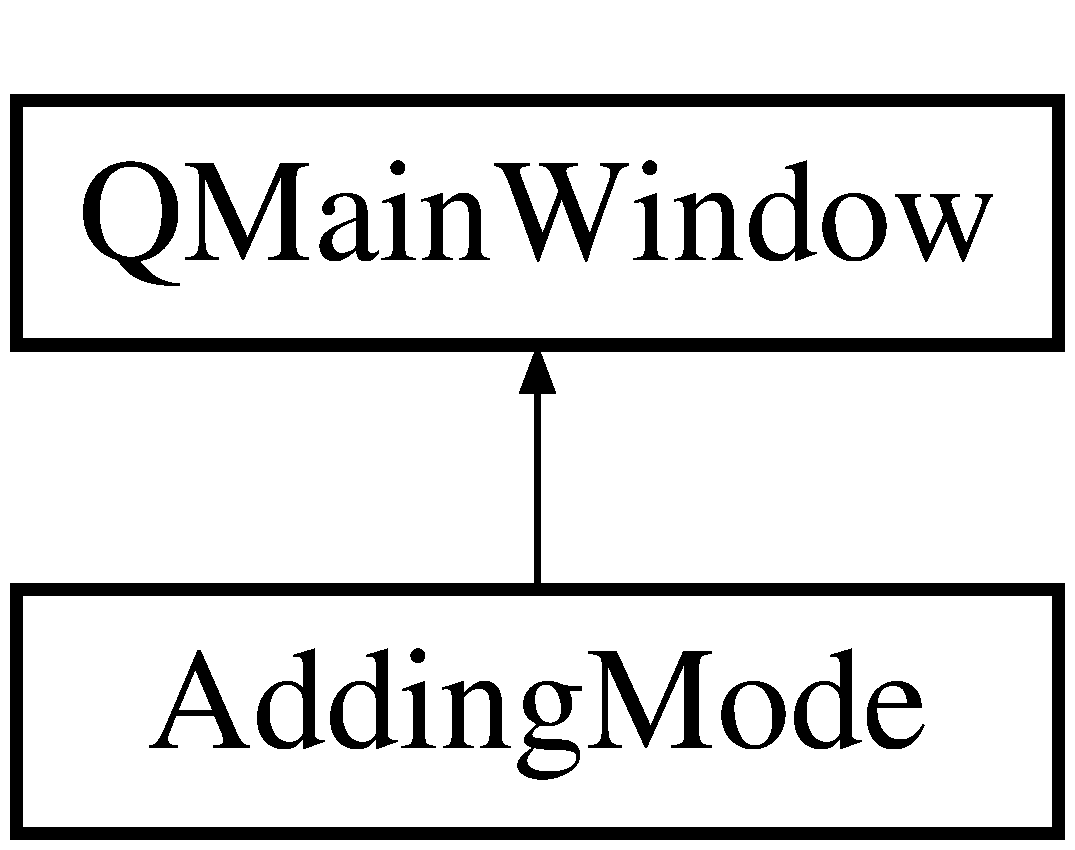
\includegraphics[height=2.000000cm]{class_adding_mode}
\end{center}
\end{figure}
\subsection*{Signals}
\begin{DoxyCompactItemize}
\item 
void \hyperlink{class_adding_mode_ac9a9d671ccfc803f9844cde060a12ca5}{show\+Event\+Planner} ()
\begin{DoxyCompactList}\small\item\em show\+Event\+Planner \end{DoxyCompactList}\end{DoxyCompactItemize}
\subsection*{Public Member Functions}
\begin{DoxyCompactItemize}
\item 
\hyperlink{class_adding_mode_aa8830870d671f8d806bedd0ecf03d065}{Adding\+Mode} (\hyperlink{class_session}{Session} $\ast$session, Q\+Widget $\ast$parent=0)
\begin{DoxyCompactList}\small\item\em \hyperlink{class_adding_mode}{Adding\+Mode}. \end{DoxyCompactList}\item 
\hyperlink{class_adding_mode_a7006861b4a358f4cdc704bcfe15e5a7a}{$\sim$\+Adding\+Mode} ()
\end{DoxyCompactItemize}


\subsection{Detailed Description}
The \hyperlink{class_adding_mode}{Adding\+Mode} class. 

Class for adding availablity to an event. 

\subsection{Constructor \& Destructor Documentation}
\mbox{\Hypertarget{class_adding_mode_aa8830870d671f8d806bedd0ecf03d065}\label{class_adding_mode_aa8830870d671f8d806bedd0ecf03d065}} 
\index{Adding\+Mode@{Adding\+Mode}!Adding\+Mode@{Adding\+Mode}}
\index{Adding\+Mode@{Adding\+Mode}!Adding\+Mode@{Adding\+Mode}}
\subsubsection{\texorpdfstring{Adding\+Mode()}{AddingMode()}}
{\footnotesize\ttfamily Adding\+Mode\+::\+Adding\+Mode (\begin{DoxyParamCaption}\item[{\hyperlink{class_session}{Session} $\ast$}]{session,  }\item[{Q\+Widget $\ast$}]{parent = {\ttfamily 0} }\end{DoxyParamCaption})\hspace{0.3cm}{\ttfamily [explicit]}}



\hyperlink{class_adding_mode}{Adding\+Mode}. 

Constructor for the Adding Mode 
\begin{DoxyParams}{Parameters}
{\em session} & \\
\hline
{\em parent} & \\
\hline
\end{DoxyParams}
\mbox{\Hypertarget{class_adding_mode_a7006861b4a358f4cdc704bcfe15e5a7a}\label{class_adding_mode_a7006861b4a358f4cdc704bcfe15e5a7a}} 
\index{Adding\+Mode@{Adding\+Mode}!````~Adding\+Mode@{$\sim$\+Adding\+Mode}}
\index{````~Adding\+Mode@{$\sim$\+Adding\+Mode}!Adding\+Mode@{Adding\+Mode}}
\subsubsection{\texorpdfstring{$\sim$\+Adding\+Mode()}{~AddingMode()}}
{\footnotesize\ttfamily Adding\+Mode\+::$\sim$\+Adding\+Mode (\begin{DoxyParamCaption}{ }\end{DoxyParamCaption})}



\subsection{Member Function Documentation}
\mbox{\Hypertarget{class_adding_mode_ac9a9d671ccfc803f9844cde060a12ca5}\label{class_adding_mode_ac9a9d671ccfc803f9844cde060a12ca5}} 
\index{Adding\+Mode@{Adding\+Mode}!show\+Event\+Planner@{show\+Event\+Planner}}
\index{show\+Event\+Planner@{show\+Event\+Planner}!Adding\+Mode@{Adding\+Mode}}
\subsubsection{\texorpdfstring{show\+Event\+Planner}{showEventPlanner}}
{\footnotesize\ttfamily void Adding\+Mode\+::show\+Event\+Planner (\begin{DoxyParamCaption}{ }\end{DoxyParamCaption})\hspace{0.3cm}{\ttfamily [signal]}}



show\+Event\+Planner 

Signal for switch back to the \hyperlink{class_event}{Event} Planner 

The documentation for this class was generated from the following files\+:\begin{DoxyCompactItemize}
\item 
\hyperlink{addingmode_8h}{addingmode.\+h}\item 
\hyperlink{addingmode_8cpp}{addingmode.\+cpp}\end{DoxyCompactItemize}

\hypertarget{classattendee}{}\section{attendee Class Reference}
\label{classattendee}\index{attendee@{attendee}}


{\ttfamily \#include $<$attendee.\+h$>$}

\subsection*{Public Member Functions}
\begin{DoxyCompactItemize}
\item 
\hyperlink{classattendee_a9a40f413382f38d884f549e839d597be}{attendee} ()
\begin{DoxyCompactList}\small\item\em Default constructor. \end{DoxyCompactList}\item 
\hyperlink{classattendee_a18ac0517146b42c12028c2cc7d056ca3}{attendee} (int id, Q\+String aname, Q\+List$<$ int $>$ avail)
\begin{DoxyCompactList}\small\item\em Constructor. \end{DoxyCompactList}\item 
int \hyperlink{classattendee_a401329192a983fa7ce39a23864082d9c}{get\+Event\+ID} ()
\begin{DoxyCompactList}\small\item\em get\+Event\+ID \end{DoxyCompactList}\item 
void \hyperlink{classattendee_a9342533ee9136a1714329114b2a9c114}{set\+Event\+ID} (int id)
\begin{DoxyCompactList}\small\item\em set\+Event\+ID \end{DoxyCompactList}\item 
Q\+String \hyperlink{classattendee_a7af6210007dc95cb254562f5e3ed695b}{get\+Attendee\+Name} ()
\begin{DoxyCompactList}\small\item\em get\+Attendee\+Name \end{DoxyCompactList}\item 
void \hyperlink{classattendee_a1474b7029b761e5c0bdd418d6b985ff9}{set\+Attendee\+Name} (Q\+String aname)
\begin{DoxyCompactList}\small\item\em set\+Attendee\+Name \end{DoxyCompactList}\item 
Q\+List$<$ int $>$ \hyperlink{classattendee_a2ec27aa5e40dd1bab0123f0472f2fed0}{get\+Availability} ()
\begin{DoxyCompactList}\small\item\em get\+Availability \end{DoxyCompactList}\item 
void \hyperlink{classattendee_a7f9eed27b7b780b59cbbb6931e086ee9}{set\+Availability} (Q\+List$<$ int $>$ avail)
\begin{DoxyCompactList}\small\item\em set\+Availability \end{DoxyCompactList}\item 
void \hyperlink{classattendee_a0bae1f348a38a1fc8ca67a141f8c771c}{add\+Availability} (int slot)
\begin{DoxyCompactList}\small\item\em add\+Availability \end{DoxyCompactList}\item 
Q\+String\+List \hyperlink{classattendee_a69818adb55caa399615fa43b7b7f0588}{get\+Tasks} ()
\begin{DoxyCompactList}\small\item\em get\+Tasks \end{DoxyCompactList}\item 
void \hyperlink{classattendee_a9b172bfafdfeb9b36a6b4ea1ec78537a}{set\+Tasks} (Q\+String task\+String)
\begin{DoxyCompactList}\small\item\em set\+Tasks \end{DoxyCompactList}\item 
void \hyperlink{classattendee_ac80fc3f8fb032f0b856da59aaedeecab}{add\+Task} (Q\+String task)
\begin{DoxyCompactList}\small\item\em add\+Task \end{DoxyCompactList}\end{DoxyCompactItemize}


\subsection{Constructor \& Destructor Documentation}
\mbox{\Hypertarget{classattendee_a9a40f413382f38d884f549e839d597be}\label{classattendee_a9a40f413382f38d884f549e839d597be}} 
\index{attendee@{attendee}!attendee@{attendee}}
\index{attendee@{attendee}!attendee@{attendee}}
\subsubsection{\texorpdfstring{attendee()}{attendee()}\hspace{0.1cm}{\footnotesize\ttfamily [1/2]}}
{\footnotesize\ttfamily attendee\+::attendee (\begin{DoxyParamCaption}{ }\end{DoxyParamCaption})}



Default constructor. 

\mbox{\Hypertarget{classattendee_a18ac0517146b42c12028c2cc7d056ca3}\label{classattendee_a18ac0517146b42c12028c2cc7d056ca3}} 
\index{attendee@{attendee}!attendee@{attendee}}
\index{attendee@{attendee}!attendee@{attendee}}
\subsubsection{\texorpdfstring{attendee()}{attendee()}\hspace{0.1cm}{\footnotesize\ttfamily [2/2]}}
{\footnotesize\ttfamily attendee\+::attendee (\begin{DoxyParamCaption}\item[{int}]{id,  }\item[{Q\+String}]{aname,  }\item[{Q\+List$<$ int $>$}]{avail }\end{DoxyParamCaption})}



Constructor. 

Will create a full attendee object with an eventid, name, and list of availability 
\begin{DoxyParams}{Parameters}
{\em id} & \\
\hline
{\em aname} & \\
\hline
{\em avail} & \\
\hline
\end{DoxyParams}


\subsection{Member Function Documentation}
\mbox{\Hypertarget{classattendee_a0bae1f348a38a1fc8ca67a141f8c771c}\label{classattendee_a0bae1f348a38a1fc8ca67a141f8c771c}} 
\index{attendee@{attendee}!add\+Availability@{add\+Availability}}
\index{add\+Availability@{add\+Availability}!attendee@{attendee}}
\subsubsection{\texorpdfstring{add\+Availability()}{addAvailability()}}
{\footnotesize\ttfamily void attendee\+::add\+Availability (\begin{DoxyParamCaption}\item[{int}]{slot }\end{DoxyParamCaption})}



add\+Availability 


\begin{DoxyParams}{Parameters}
{\em slot} & to add to availability list \\
\hline
\end{DoxyParams}
\mbox{\Hypertarget{classattendee_ac80fc3f8fb032f0b856da59aaedeecab}\label{classattendee_ac80fc3f8fb032f0b856da59aaedeecab}} 
\index{attendee@{attendee}!add\+Task@{add\+Task}}
\index{add\+Task@{add\+Task}!attendee@{attendee}}
\subsubsection{\texorpdfstring{add\+Task()}{addTask()}}
{\footnotesize\ttfamily void attendee\+::add\+Task (\begin{DoxyParamCaption}\item[{Q\+String}]{task }\end{DoxyParamCaption})}



add\+Task 

Adds a Q\+String task to the list of tasks 
\begin{DoxyParams}{Parameters}
{\em task} & \\
\hline
\end{DoxyParams}
\mbox{\Hypertarget{classattendee_a7af6210007dc95cb254562f5e3ed695b}\label{classattendee_a7af6210007dc95cb254562f5e3ed695b}} 
\index{attendee@{attendee}!get\+Attendee\+Name@{get\+Attendee\+Name}}
\index{get\+Attendee\+Name@{get\+Attendee\+Name}!attendee@{attendee}}
\subsubsection{\texorpdfstring{get\+Attendee\+Name()}{getAttendeeName()}}
{\footnotesize\ttfamily Q\+String attendee\+::get\+Attendee\+Name (\begin{DoxyParamCaption}{ }\end{DoxyParamCaption})}



get\+Attendee\+Name 

\begin{DoxyReturn}{Returns}
Q\+String attendee name 
\end{DoxyReturn}
\mbox{\Hypertarget{classattendee_a2ec27aa5e40dd1bab0123f0472f2fed0}\label{classattendee_a2ec27aa5e40dd1bab0123f0472f2fed0}} 
\index{attendee@{attendee}!get\+Availability@{get\+Availability}}
\index{get\+Availability@{get\+Availability}!attendee@{attendee}}
\subsubsection{\texorpdfstring{get\+Availability()}{getAvailability()}}
{\footnotesize\ttfamily Q\+List$<$ int $>$ attendee\+::get\+Availability (\begin{DoxyParamCaption}{ }\end{DoxyParamCaption})}



get\+Availability 

\begin{DoxyReturn}{Returns}
List of ints with user availability 
\end{DoxyReturn}
\mbox{\Hypertarget{classattendee_a401329192a983fa7ce39a23864082d9c}\label{classattendee_a401329192a983fa7ce39a23864082d9c}} 
\index{attendee@{attendee}!get\+Event\+ID@{get\+Event\+ID}}
\index{get\+Event\+ID@{get\+Event\+ID}!attendee@{attendee}}
\subsubsection{\texorpdfstring{get\+Event\+I\+D()}{getEventID()}}
{\footnotesize\ttfamily int attendee\+::get\+Event\+ID (\begin{DoxyParamCaption}{ }\end{DoxyParamCaption})}



get\+Event\+ID 

\begin{DoxyReturn}{Returns}
int ID of event 
\end{DoxyReturn}
\mbox{\Hypertarget{classattendee_a69818adb55caa399615fa43b7b7f0588}\label{classattendee_a69818adb55caa399615fa43b7b7f0588}} 
\index{attendee@{attendee}!get\+Tasks@{get\+Tasks}}
\index{get\+Tasks@{get\+Tasks}!attendee@{attendee}}
\subsubsection{\texorpdfstring{get\+Tasks()}{getTasks()}}
{\footnotesize\ttfamily Q\+String\+List attendee\+::get\+Tasks (\begin{DoxyParamCaption}{ }\end{DoxyParamCaption})}



get\+Tasks 

\begin{DoxyReturn}{Returns}
Q\+String\+List of tasks 
\end{DoxyReturn}
\mbox{\Hypertarget{classattendee_a1474b7029b761e5c0bdd418d6b985ff9}\label{classattendee_a1474b7029b761e5c0bdd418d6b985ff9}} 
\index{attendee@{attendee}!set\+Attendee\+Name@{set\+Attendee\+Name}}
\index{set\+Attendee\+Name@{set\+Attendee\+Name}!attendee@{attendee}}
\subsubsection{\texorpdfstring{set\+Attendee\+Name()}{setAttendeeName()}}
{\footnotesize\ttfamily void attendee\+::set\+Attendee\+Name (\begin{DoxyParamCaption}\item[{Q\+String}]{aname }\end{DoxyParamCaption})}



set\+Attendee\+Name 


\begin{DoxyParams}{Parameters}
{\em name} & of event \\
\hline
\end{DoxyParams}
\mbox{\Hypertarget{classattendee_a7f9eed27b7b780b59cbbb6931e086ee9}\label{classattendee_a7f9eed27b7b780b59cbbb6931e086ee9}} 
\index{attendee@{attendee}!set\+Availability@{set\+Availability}}
\index{set\+Availability@{set\+Availability}!attendee@{attendee}}
\subsubsection{\texorpdfstring{set\+Availability()}{setAvailability()}}
{\footnotesize\ttfamily void attendee\+::set\+Availability (\begin{DoxyParamCaption}\item[{Q\+List$<$ int $>$}]{avail }\end{DoxyParamCaption})}



set\+Availability 


\begin{DoxyParams}{Parameters}
{\em avail} & of user for event id \\
\hline
\end{DoxyParams}
\mbox{\Hypertarget{classattendee_a9342533ee9136a1714329114b2a9c114}\label{classattendee_a9342533ee9136a1714329114b2a9c114}} 
\index{attendee@{attendee}!set\+Event\+ID@{set\+Event\+ID}}
\index{set\+Event\+ID@{set\+Event\+ID}!attendee@{attendee}}
\subsubsection{\texorpdfstring{set\+Event\+I\+D()}{setEventID()}}
{\footnotesize\ttfamily void attendee\+::set\+Event\+ID (\begin{DoxyParamCaption}\item[{int}]{id }\end{DoxyParamCaption})}



set\+Event\+ID 


\begin{DoxyParams}{Parameters}
{\em id} & of event \\
\hline
\end{DoxyParams}
\mbox{\Hypertarget{classattendee_a9b172bfafdfeb9b36a6b4ea1ec78537a}\label{classattendee_a9b172bfafdfeb9b36a6b4ea1ec78537a}} 
\index{attendee@{attendee}!set\+Tasks@{set\+Tasks}}
\index{set\+Tasks@{set\+Tasks}!attendee@{attendee}}
\subsubsection{\texorpdfstring{set\+Tasks()}{setTasks()}}
{\footnotesize\ttfamily void attendee\+::set\+Tasks (\begin{DoxyParamCaption}\item[{Q\+String}]{task\+String }\end{DoxyParamCaption})}



set\+Tasks 


\begin{DoxyParams}{Parameters}
{\em task\+String} & String of semi-\/colon separated task strings \\
\hline
\end{DoxyParams}


The documentation for this class was generated from the following files\+:\begin{DoxyCompactItemize}
\item 
\hyperlink{attendee_8h}{attendee.\+h}\item 
\hyperlink{attendee_8cpp}{attendee.\+cpp}\end{DoxyCompactItemize}

\hypertarget{class_event}{}\section{Event Class Reference}
\label{class_event}\index{Event@{Event}}


The \hyperlink{class_event}{Event} class.  




{\ttfamily \#include $<$event.\+h$>$}

\subsection*{Public Member Functions}
\begin{DoxyCompactItemize}
\item 
\hyperlink{class_event_a5a40dd4708297f7031e29b39e039ae10}{Event} ()
\begin{DoxyCompactList}\small\item\em \hyperlink{class_event}{Event}. \end{DoxyCompactList}\item 
\hyperlink{class_event_a7d7306f5661b66b543be76e849f20329}{Event} (Q\+String owner, Q\+String event\+Name, int event\+ID, Q\+String\+List days, Q\+String\+List tasks, Q\+List$<$ int $>$ timeslots)
\begin{DoxyCompactList}\small\item\em \hyperlink{class_event}{Event}. \end{DoxyCompactList}\item 
\hyperlink{class_event_a7704ec01ce91e673885792054214b3d2}{$\sim$\+Event} ()
\item 
void \hyperlink{class_event_a0cc103761f52f4a7c2e4d935c8e0809e}{set\+Days} (Q\+String day\+String)
\begin{DoxyCompactList}\small\item\em set\+Days \end{DoxyCompactList}\item 
Q\+String\+List \hyperlink{class_event_ac8aac8eac691a08cf0822a380fe29eb2}{get\+Days} ()
\begin{DoxyCompactList}\small\item\em get\+Day \end{DoxyCompactList}\item 
void \hyperlink{class_event_a23cb6c79d76f416edcbdc2044fa73138}{set\+Tasks} (Q\+String tasks)
\begin{DoxyCompactList}\small\item\em set\+Tasks \end{DoxyCompactList}\item 
Q\+String\+List \hyperlink{class_event_afd035786dd05f97c7a820878444306f6}{get\+Tasks} ()
\begin{DoxyCompactList}\small\item\em get\+Tasks \end{DoxyCompactList}\item 
bool \hyperlink{class_event_a81270b85694de5ceaa79ae4e6588d000}{remove\+Task} (Q\+String task)
\begin{DoxyCompactList}\small\item\em remove\+Task \end{DoxyCompactList}\item 
Q\+String \hyperlink{class_event_a2846f2dfad84c083d829fdf3d915c05a}{get\+Event\+Name} ()
\begin{DoxyCompactList}\small\item\em get\+Event\+Name \end{DoxyCompactList}\item 
void \hyperlink{class_event_a15b675acab68dd6a840421ec72aeef57}{set\+Event\+Name} (Q\+String event\+Name)
\begin{DoxyCompactList}\small\item\em set\+Event\+Name \end{DoxyCompactList}\item 
Q\+String \hyperlink{class_event_ab7e1dc08bd691aaf95ad994afdea6d2b}{get\+Owner} () const
\begin{DoxyCompactList}\small\item\em get\+Owner \end{DoxyCompactList}\item 
void \hyperlink{class_event_a4c5b75b1d4c162cb7489ee6a4ced8af0}{set\+Owner} (Q\+String owner)
\begin{DoxyCompactList}\small\item\em set\+Owner \end{DoxyCompactList}\item 
Q\+List$<$ int $>$ \hyperlink{class_event_ae105da8497f73e20c687060c5837e6f8}{get\+Time\+Slots} ()
\begin{DoxyCompactList}\small\item\em get\+Time\+Slots \end{DoxyCompactList}\item 
void \hyperlink{class_event_ad39ee28106d13c32165cb091a500f896}{set\+Time\+Slots} (Q\+List$<$ int $>$ time\+Slots)
\begin{DoxyCompactList}\small\item\em set\+Time\+Slots \end{DoxyCompactList}\item 
Q\+String \hyperlink{class_event_ab2c59affdf5f762ecedd77a689ba08de}{print\+Event} ()
\begin{DoxyCompactList}\small\item\em print\+Event \end{DoxyCompactList}\item 
int \hyperlink{class_event_a019343d5fbe993108f49362f134ef746}{get\+ID} () const
\begin{DoxyCompactList}\small\item\em get\+ID \end{DoxyCompactList}\item 
void \hyperlink{class_event_a3c90e712012a92068a2fb14e302de0be}{set\+ID} (int ID)
\begin{DoxyCompactList}\small\item\em set\+ID \end{DoxyCompactList}\item 
Q\+List$<$ \hyperlink{classattendee}{attendee} $\ast$ $>$ \hyperlink{class_event_a56f9898f75ae301df1d10523de57f500}{get\+Attendees} ()
\begin{DoxyCompactList}\small\item\em get\+Attendees \end{DoxyCompactList}\item 
Q\+String\+List \hyperlink{class_event_adb10c77700599fb4c6047fd8f4476beb}{get\+Attendees\+At\+Timeslot} (int timeslot)
\begin{DoxyCompactList}\small\item\em get\+Attendees\+At\+Timeslot \end{DoxyCompactList}\item 
void \hyperlink{class_event_af632e4550dcd4eb70c5a45c57af615b7}{set\+Attendees} (Q\+List$<$ \hyperlink{classattendee}{attendee} $\ast$$>$)
\begin{DoxyCompactList}\small\item\em set\+Attendees \end{DoxyCompactList}\item 
void \hyperlink{class_event_a0940f63f5ac2324d7c61e204ed782bd0}{add\+Attendee} (Q\+String name, int slot)
\begin{DoxyCompactList}\small\item\em add\+Attendee \end{DoxyCompactList}\item 
void \hyperlink{class_event_a7be36f174942f39cab6917d09e139a14}{add\+Attendee} (\hyperlink{classattendee}{attendee} $\ast$attn)
\begin{DoxyCompactList}\small\item\em add\+Attendee \end{DoxyCompactList}\item 
void \hyperlink{class_event_abd8ba2203b1fc2e1c66280ed2d63adda}{add\+Attendee} (Q\+String name, Q\+List$<$ int $>$ slot)
\begin{DoxyCompactList}\small\item\em add\+Attendee \end{DoxyCompactList}\item 
int \hyperlink{class_event_ac06e3e571247a3804491b14301b045d3}{has\+Attendee} (Q\+String name)
\begin{DoxyCompactList}\small\item\em has\+Attendee \end{DoxyCompactList}\end{DoxyCompactItemize}


\subsection{Detailed Description}
The \hyperlink{class_event}{Event} class. 

Class used to store details of an event. 

\subsection{Constructor \& Destructor Documentation}
\mbox{\Hypertarget{class_event_a5a40dd4708297f7031e29b39e039ae10}\label{class_event_a5a40dd4708297f7031e29b39e039ae10}} 
\index{Event@{Event}!Event@{Event}}
\index{Event@{Event}!Event@{Event}}
\subsubsection{\texorpdfstring{Event()}{Event()}\hspace{0.1cm}{\footnotesize\ttfamily [1/2]}}
{\footnotesize\ttfamily Event\+::\+Event (\begin{DoxyParamCaption}{ }\end{DoxyParamCaption})}



\hyperlink{class_event}{Event}. 

Default constructor. Only default initilizations are made. \mbox{\Hypertarget{class_event_a7d7306f5661b66b543be76e849f20329}\label{class_event_a7d7306f5661b66b543be76e849f20329}} 
\index{Event@{Event}!Event@{Event}}
\index{Event@{Event}!Event@{Event}}
\subsubsection{\texorpdfstring{Event()}{Event()}\hspace{0.1cm}{\footnotesize\ttfamily [2/2]}}
{\footnotesize\ttfamily Event\+::\+Event (\begin{DoxyParamCaption}\item[{Q\+String}]{owner,  }\item[{Q\+String}]{event\+Name,  }\item[{int}]{event\+ID,  }\item[{Q\+String\+List}]{days,  }\item[{Q\+String\+List}]{tasks,  }\item[{Q\+List$<$ int $>$}]{timeslots }\end{DoxyParamCaption})}



\hyperlink{class_event}{Event}. 

Constructor used to create fully initialized \hyperlink{class_event}{Event} object. 
\begin{DoxyParams}{Parameters}
{\em owner} & Name of the creator \\
\hline
{\em event\+Name} & Name of the event \\
\hline
{\em event\+ID} & \hyperlink{class_event}{Event}\textquotesingle{}s ID \\
\hline
{\em days} & List of days of format \textquotesingle{}M\+M-\/\+D\+D-\/\+Y\+Y\+YY\textquotesingle{} that it spans \\
\hline
{\em tasks} & List of tasks that have not been fulfilled \\
\hline
{\em timeslots} & List of timeslots that range from 0 -\/ ((number of days $\ast$ 48) -\/ 1) \\
\hline
\end{DoxyParams}
\mbox{\Hypertarget{class_event_a7704ec01ce91e673885792054214b3d2}\label{class_event_a7704ec01ce91e673885792054214b3d2}} 
\index{Event@{Event}!````~Event@{$\sim$\+Event}}
\index{````~Event@{$\sim$\+Event}!Event@{Event}}
\subsubsection{\texorpdfstring{$\sim$\+Event()}{~Event()}}
{\footnotesize\ttfamily Event\+::$\sim$\+Event (\begin{DoxyParamCaption}{ }\end{DoxyParamCaption})}



\subsection{Member Function Documentation}
\mbox{\Hypertarget{class_event_a0940f63f5ac2324d7c61e204ed782bd0}\label{class_event_a0940f63f5ac2324d7c61e204ed782bd0}} 
\index{Event@{Event}!add\+Attendee@{add\+Attendee}}
\index{add\+Attendee@{add\+Attendee}!Event@{Event}}
\subsubsection{\texorpdfstring{add\+Attendee()}{addAttendee()}\hspace{0.1cm}{\footnotesize\ttfamily [1/3]}}
{\footnotesize\ttfamily void Event\+::add\+Attendee (\begin{DoxyParamCaption}\item[{Q\+String}]{name,  }\item[{int}]{slot }\end{DoxyParamCaption})}



add\+Attendee 


\begin{DoxyParams}{Parameters}
{\em name} & \\
\hline
{\em slot} & \\
\hline
\end{DoxyParams}
\mbox{\Hypertarget{class_event_a7be36f174942f39cab6917d09e139a14}\label{class_event_a7be36f174942f39cab6917d09e139a14}} 
\index{Event@{Event}!add\+Attendee@{add\+Attendee}}
\index{add\+Attendee@{add\+Attendee}!Event@{Event}}
\subsubsection{\texorpdfstring{add\+Attendee()}{addAttendee()}\hspace{0.1cm}{\footnotesize\ttfamily [2/3]}}
{\footnotesize\ttfamily void Event\+::add\+Attendee (\begin{DoxyParamCaption}\item[{\hyperlink{classattendee}{attendee} $\ast$}]{attn }\end{DoxyParamCaption})}



add\+Attendee 


\begin{DoxyParams}{Parameters}
{\em attn} & \\
\hline
\end{DoxyParams}
\mbox{\Hypertarget{class_event_abd8ba2203b1fc2e1c66280ed2d63adda}\label{class_event_abd8ba2203b1fc2e1c66280ed2d63adda}} 
\index{Event@{Event}!add\+Attendee@{add\+Attendee}}
\index{add\+Attendee@{add\+Attendee}!Event@{Event}}
\subsubsection{\texorpdfstring{add\+Attendee()}{addAttendee()}\hspace{0.1cm}{\footnotesize\ttfamily [3/3]}}
{\footnotesize\ttfamily void Event\+::add\+Attendee (\begin{DoxyParamCaption}\item[{Q\+String}]{name,  }\item[{Q\+List$<$ int $>$}]{slot }\end{DoxyParamCaption})}



add\+Attendee 


\begin{DoxyParams}{Parameters}
{\em name} & \\
\hline
{\em slots} & \\
\hline
\end{DoxyParams}
\mbox{\Hypertarget{class_event_a56f9898f75ae301df1d10523de57f500}\label{class_event_a56f9898f75ae301df1d10523de57f500}} 
\index{Event@{Event}!get\+Attendees@{get\+Attendees}}
\index{get\+Attendees@{get\+Attendees}!Event@{Event}}
\subsubsection{\texorpdfstring{get\+Attendees()}{getAttendees()}}
{\footnotesize\ttfamily Q\+List$<$ \hyperlink{classattendee}{attendee} $\ast$ $>$ Event\+::get\+Attendees (\begin{DoxyParamCaption}{ }\end{DoxyParamCaption})}



get\+Attendees 

\begin{DoxyReturn}{Returns}

\end{DoxyReturn}
\mbox{\Hypertarget{class_event_adb10c77700599fb4c6047fd8f4476beb}\label{class_event_adb10c77700599fb4c6047fd8f4476beb}} 
\index{Event@{Event}!get\+Attendees\+At\+Timeslot@{get\+Attendees\+At\+Timeslot}}
\index{get\+Attendees\+At\+Timeslot@{get\+Attendees\+At\+Timeslot}!Event@{Event}}
\subsubsection{\texorpdfstring{get\+Attendees\+At\+Timeslot()}{getAttendeesAtTimeslot()}}
{\footnotesize\ttfamily Q\+String\+List Event\+::get\+Attendees\+At\+Timeslot (\begin{DoxyParamCaption}\item[{int}]{timeslot }\end{DoxyParamCaption})}



get\+Attendees\+At\+Timeslot 


\begin{DoxyParams}{Parameters}
{\em timeslot} & \\
\hline
\end{DoxyParams}
\begin{DoxyReturn}{Returns}

\end{DoxyReturn}
\mbox{\Hypertarget{class_event_ac8aac8eac691a08cf0822a380fe29eb2}\label{class_event_ac8aac8eac691a08cf0822a380fe29eb2}} 
\index{Event@{Event}!get\+Days@{get\+Days}}
\index{get\+Days@{get\+Days}!Event@{Event}}
\subsubsection{\texorpdfstring{get\+Days()}{getDays()}}
{\footnotesize\ttfamily Q\+String\+List Event\+::get\+Days (\begin{DoxyParamCaption}{ }\end{DoxyParamCaption})}



get\+Day 

Returns the date of the event \begin{DoxyReturn}{Returns}
Q\+String\+List of Q\+String with format \char`\"{}\+M\+M-\/\+D\+D-\/\+Y\+Y\+Y\+Y\char`\"{} 
\end{DoxyReturn}
\mbox{\Hypertarget{class_event_a2846f2dfad84c083d829fdf3d915c05a}\label{class_event_a2846f2dfad84c083d829fdf3d915c05a}} 
\index{Event@{Event}!get\+Event\+Name@{get\+Event\+Name}}
\index{get\+Event\+Name@{get\+Event\+Name}!Event@{Event}}
\subsubsection{\texorpdfstring{get\+Event\+Name()}{getEventName()}}
{\footnotesize\ttfamily Q\+String Event\+::get\+Event\+Name (\begin{DoxyParamCaption}{ }\end{DoxyParamCaption})}



get\+Event\+Name 

Returns the name of the event. \begin{DoxyReturn}{Returns}
Q\+String 
\end{DoxyReturn}
\mbox{\Hypertarget{class_event_a019343d5fbe993108f49362f134ef746}\label{class_event_a019343d5fbe993108f49362f134ef746}} 
\index{Event@{Event}!get\+ID@{get\+ID}}
\index{get\+ID@{get\+ID}!Event@{Event}}
\subsubsection{\texorpdfstring{get\+I\+D()}{getID()}}
{\footnotesize\ttfamily int Event\+::get\+ID (\begin{DoxyParamCaption}{ }\end{DoxyParamCaption}) const}



get\+ID 

\begin{DoxyReturn}{Returns}
int Event\+ID 
\end{DoxyReturn}
\mbox{\Hypertarget{class_event_ab7e1dc08bd691aaf95ad994afdea6d2b}\label{class_event_ab7e1dc08bd691aaf95ad994afdea6d2b}} 
\index{Event@{Event}!get\+Owner@{get\+Owner}}
\index{get\+Owner@{get\+Owner}!Event@{Event}}
\subsubsection{\texorpdfstring{get\+Owner()}{getOwner()}}
{\footnotesize\ttfamily Q\+String Event\+::get\+Owner (\begin{DoxyParamCaption}{ }\end{DoxyParamCaption}) const}



get\+Owner 

Returns the name of the person who created the event. \begin{DoxyReturn}{Returns}
Q\+String 
\end{DoxyReturn}
\mbox{\Hypertarget{class_event_afd035786dd05f97c7a820878444306f6}\label{class_event_afd035786dd05f97c7a820878444306f6}} 
\index{Event@{Event}!get\+Tasks@{get\+Tasks}}
\index{get\+Tasks@{get\+Tasks}!Event@{Event}}
\subsubsection{\texorpdfstring{get\+Tasks()}{getTasks()}}
{\footnotesize\ttfamily Q\+String\+List Event\+::get\+Tasks (\begin{DoxyParamCaption}{ }\end{DoxyParamCaption})}



get\+Tasks 

\begin{DoxyReturn}{Returns}
Q\+String\+List of tasks 
\end{DoxyReturn}
\mbox{\Hypertarget{class_event_ae105da8497f73e20c687060c5837e6f8}\label{class_event_ae105da8497f73e20c687060c5837e6f8}} 
\index{Event@{Event}!get\+Time\+Slots@{get\+Time\+Slots}}
\index{get\+Time\+Slots@{get\+Time\+Slots}!Event@{Event}}
\subsubsection{\texorpdfstring{get\+Time\+Slots()}{getTimeSlots()}}
{\footnotesize\ttfamily Q\+List$<$ int $>$ Event\+::get\+Time\+Slots (\begin{DoxyParamCaption}{ }\end{DoxyParamCaption})}



get\+Time\+Slots 

Returns the private member Q\+List$<$\+Time\+Slot$>$ time\+Slots. \begin{DoxyReturn}{Returns}
Q\+List$<$\+Time\+Slot$>$ 
\end{DoxyReturn}
\mbox{\Hypertarget{class_event_ac06e3e571247a3804491b14301b045d3}\label{class_event_ac06e3e571247a3804491b14301b045d3}} 
\index{Event@{Event}!has\+Attendee@{has\+Attendee}}
\index{has\+Attendee@{has\+Attendee}!Event@{Event}}
\subsubsection{\texorpdfstring{has\+Attendee()}{hasAttendee()}}
{\footnotesize\ttfamily int Event\+::has\+Attendee (\begin{DoxyParamCaption}\item[{Q\+String}]{name }\end{DoxyParamCaption})}



has\+Attendee 


\begin{DoxyParams}{Parameters}
{\em name} & \\
\hline
\end{DoxyParams}
\begin{DoxyReturn}{Returns}
-\/1 if no attendee has matching name, otherwise returns the index of the attendee 
\end{DoxyReturn}
\mbox{\Hypertarget{class_event_ab2c59affdf5f762ecedd77a689ba08de}\label{class_event_ab2c59affdf5f762ecedd77a689ba08de}} 
\index{Event@{Event}!print\+Event@{print\+Event}}
\index{print\+Event@{print\+Event}!Event@{Event}}
\subsubsection{\texorpdfstring{print\+Event()}{printEvent()}}
{\footnotesize\ttfamily Q\+String Event\+::print\+Event (\begin{DoxyParamCaption}{ }\end{DoxyParamCaption})}



print\+Event 

A formatted Q\+String with the Owner, \hyperlink{class_event}{Event} Name, and Date \begin{DoxyReturn}{Returns}
Q\+String 
\end{DoxyReturn}
\mbox{\Hypertarget{class_event_a81270b85694de5ceaa79ae4e6588d000}\label{class_event_a81270b85694de5ceaa79ae4e6588d000}} 
\index{Event@{Event}!remove\+Task@{remove\+Task}}
\index{remove\+Task@{remove\+Task}!Event@{Event}}
\subsubsection{\texorpdfstring{remove\+Task()}{removeTask()}}
{\footnotesize\ttfamily bool Event\+::remove\+Task (\begin{DoxyParamCaption}\item[{Q\+String}]{task }\end{DoxyParamCaption})}



remove\+Task 


\begin{DoxyParams}{Parameters}
{\em task} & to be removed \\
\hline
\end{DoxyParams}
\begin{DoxyReturn}{Returns}
true if the task was successfully removed 
\end{DoxyReturn}
\mbox{\Hypertarget{class_event_af632e4550dcd4eb70c5a45c57af615b7}\label{class_event_af632e4550dcd4eb70c5a45c57af615b7}} 
\index{Event@{Event}!set\+Attendees@{set\+Attendees}}
\index{set\+Attendees@{set\+Attendees}!Event@{Event}}
\subsubsection{\texorpdfstring{set\+Attendees()}{setAttendees()}}
{\footnotesize\ttfamily void Event\+::set\+Attendees (\begin{DoxyParamCaption}\item[{Q\+List$<$ \hyperlink{classattendee}{attendee} $\ast$$>$}]{a\+List }\end{DoxyParamCaption})}



set\+Attendees 

\mbox{\Hypertarget{class_event_a0cc103761f52f4a7c2e4d935c8e0809e}\label{class_event_a0cc103761f52f4a7c2e4d935c8e0809e}} 
\index{Event@{Event}!set\+Days@{set\+Days}}
\index{set\+Days@{set\+Days}!Event@{Event}}
\subsubsection{\texorpdfstring{set\+Days()}{setDays()}}
{\footnotesize\ttfamily void Event\+::set\+Days (\begin{DoxyParamCaption}\item[{Q\+String}]{day\+String }\end{DoxyParamCaption})}



set\+Days 


\begin{DoxyParams}{Parameters}
{\em day\+String} & \\
\hline
\end{DoxyParams}
Takes list of comma separated days of format \textquotesingle{}M\+M-\/\+D\+D-\/\+Y\+Y\+YY\textquotesingle{} and separates it into a list \mbox{\Hypertarget{class_event_a15b675acab68dd6a840421ec72aeef57}\label{class_event_a15b675acab68dd6a840421ec72aeef57}} 
\index{Event@{Event}!set\+Event\+Name@{set\+Event\+Name}}
\index{set\+Event\+Name@{set\+Event\+Name}!Event@{Event}}
\subsubsection{\texorpdfstring{set\+Event\+Name()}{setEventName()}}
{\footnotesize\ttfamily void Event\+::set\+Event\+Name (\begin{DoxyParamCaption}\item[{Q\+String}]{event\+Name }\end{DoxyParamCaption})}



set\+Event\+Name 

Sets private variable event\+Name to the passed Q\+String. 
\begin{DoxyParams}{Parameters}
{\em event\+Name} & \\
\hline
\end{DoxyParams}
\mbox{\Hypertarget{class_event_a3c90e712012a92068a2fb14e302de0be}\label{class_event_a3c90e712012a92068a2fb14e302de0be}} 
\index{Event@{Event}!set\+ID@{set\+ID}}
\index{set\+ID@{set\+ID}!Event@{Event}}
\subsubsection{\texorpdfstring{set\+I\+D()}{setID()}}
{\footnotesize\ttfamily void Event\+::set\+ID (\begin{DoxyParamCaption}\item[{int}]{ID }\end{DoxyParamCaption})}



set\+ID 


\begin{DoxyParams}{Parameters}
{\em ID} & \hyperlink{class_event}{Event} ID \\
\hline
\end{DoxyParams}
\mbox{\Hypertarget{class_event_a4c5b75b1d4c162cb7489ee6a4ced8af0}\label{class_event_a4c5b75b1d4c162cb7489ee6a4ced8af0}} 
\index{Event@{Event}!set\+Owner@{set\+Owner}}
\index{set\+Owner@{set\+Owner}!Event@{Event}}
\subsubsection{\texorpdfstring{set\+Owner()}{setOwner()}}
{\footnotesize\ttfamily void Event\+::set\+Owner (\begin{DoxyParamCaption}\item[{Q\+String}]{owner }\end{DoxyParamCaption})}



set\+Owner 

Sets private variable owner to the passed Q\+String. 
\begin{DoxyParams}{Parameters}
{\em owner} & \\
\hline
\end{DoxyParams}
\mbox{\Hypertarget{class_event_a23cb6c79d76f416edcbdc2044fa73138}\label{class_event_a23cb6c79d76f416edcbdc2044fa73138}} 
\index{Event@{Event}!set\+Tasks@{set\+Tasks}}
\index{set\+Tasks@{set\+Tasks}!Event@{Event}}
\subsubsection{\texorpdfstring{set\+Tasks()}{setTasks()}}
{\footnotesize\ttfamily void Event\+::set\+Tasks (\begin{DoxyParamCaption}\item[{Q\+String}]{tasks }\end{DoxyParamCaption})}



set\+Tasks 

Takes a list of semi-\/colon separated strings and splits it into a list 
\begin{DoxyParams}{Parameters}
{\em tasks} & \\
\hline
\end{DoxyParams}
\mbox{\Hypertarget{class_event_ad39ee28106d13c32165cb091a500f896}\label{class_event_ad39ee28106d13c32165cb091a500f896}} 
\index{Event@{Event}!set\+Time\+Slots@{set\+Time\+Slots}}
\index{set\+Time\+Slots@{set\+Time\+Slots}!Event@{Event}}
\subsubsection{\texorpdfstring{set\+Time\+Slots()}{setTimeSlots()}}
{\footnotesize\ttfamily void Event\+::set\+Time\+Slots (\begin{DoxyParamCaption}\item[{Q\+List$<$ int $>$}]{time\+Slots }\end{DoxyParamCaption})}



set\+Time\+Slots 

Sets private variable time\+Slots to the passed Q\+List$<$\+Time\+Slot$>$. 
\begin{DoxyParams}{Parameters}
{\em time\+Slots} & \\
\hline
\end{DoxyParams}


The documentation for this class was generated from the following files\+:\begin{DoxyCompactItemize}
\item 
\hyperlink{event_8h}{event.\+h}\item 
\hyperlink{event_8cpp}{event.\+cpp}\end{DoxyCompactItemize}

\hypertarget{class_event_admin_mode}{}\section{Event\+Admin\+Mode Class Reference}
\label{class_event_admin_mode}\index{Event\+Admin\+Mode@{Event\+Admin\+Mode}}


The \hyperlink{class_event_admin_mode}{Event\+Admin\+Mode} class.  




{\ttfamily \#include $<$eventadminmode.\+h$>$}

Inheritance diagram for Event\+Admin\+Mode\+:\begin{figure}[H]
\begin{center}
\leavevmode
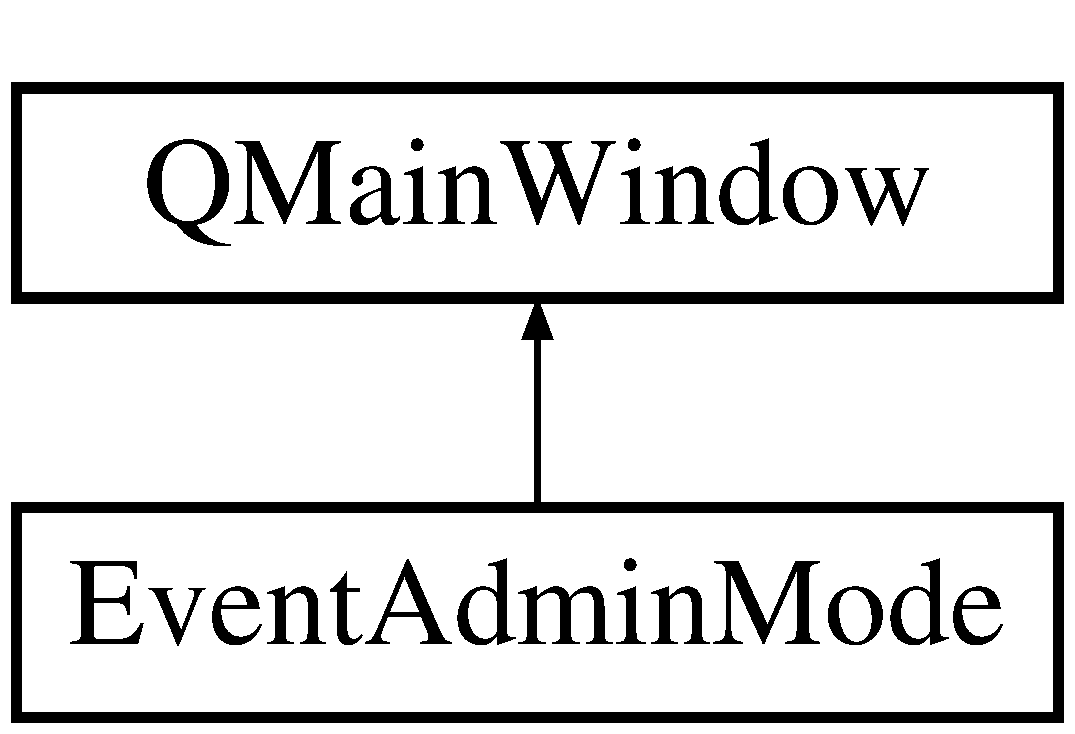
\includegraphics[height=2.000000cm]{class_event_admin_mode}
\end{center}
\end{figure}
\subsection*{Signals}
\begin{DoxyCompactItemize}
\item 
void \hyperlink{class_event_admin_mode_aff26ca6ac01a61846ccef0e55cc274de}{show\+Event\+Planner} ()
\begin{DoxyCompactList}\small\item\em show\+Event\+Planner \end{DoxyCompactList}\item 
void \hyperlink{class_event_admin_mode_a5fcf257db5008a3f634c3fcd13f06994}{quit} ()
\begin{DoxyCompactList}\small\item\em quit \end{DoxyCompactList}\end{DoxyCompactItemize}
\subsection*{Public Member Functions}
\begin{DoxyCompactItemize}
\item 
\hyperlink{class_event_admin_mode_a6f7d4e143b04287d436e9be16324626d}{Event\+Admin\+Mode} (\hyperlink{class_session}{Session} $\ast$session, Q\+Widget $\ast$parent=0)
\begin{DoxyCompactList}\small\item\em \hyperlink{class_event_admin_mode}{Event\+Admin\+Mode}. \end{DoxyCompactList}\item 
\hyperlink{class_event_admin_mode_a8b5cc3b5ad2067b0f97d7764d2520ca9}{$\sim$\+Event\+Admin\+Mode} ()
\item 
Q\+String \hyperlink{class_event_admin_mode_a22d5e21b4a4450e1917085c2375239c9}{Info\+\_\+\+Collect} (Q\+String \&Event\+Name, Q\+String person\+\_\+name, int month, int day, int year)
\begin{DoxyCompactList}\small\item\em Info\+\_\+\+Collect. \end{DoxyCompactList}\item 
void \hyperlink{class_event_admin_mode_a8e7abbf82a05352cacc29d544a682139}{set\+Style\+\_\+calendar\+Widget} ()
\begin{DoxyCompactList}\small\item\em set\+Style\+\_\+calendar\+Widget \end{DoxyCompactList}\end{DoxyCompactItemize}


\subsection{Detailed Description}
The \hyperlink{class_event_admin_mode}{Event\+Admin\+Mode} class. 

Window used for creating new events. 

\subsection{Constructor \& Destructor Documentation}
\mbox{\Hypertarget{class_event_admin_mode_a6f7d4e143b04287d436e9be16324626d}\label{class_event_admin_mode_a6f7d4e143b04287d436e9be16324626d}} 
\index{Event\+Admin\+Mode@{Event\+Admin\+Mode}!Event\+Admin\+Mode@{Event\+Admin\+Mode}}
\index{Event\+Admin\+Mode@{Event\+Admin\+Mode}!Event\+Admin\+Mode@{Event\+Admin\+Mode}}
\subsubsection{\texorpdfstring{Event\+Admin\+Mode()}{EventAdminMode()}}
{\footnotesize\ttfamily Event\+Admin\+Mode\+::\+Event\+Admin\+Mode (\begin{DoxyParamCaption}\item[{\hyperlink{class_session}{Session} $\ast$}]{session,  }\item[{Q\+Widget $\ast$}]{parent = {\ttfamily 0} }\end{DoxyParamCaption})\hspace{0.3cm}{\ttfamily [explicit]}}



\hyperlink{class_event_admin_mode}{Event\+Admin\+Mode}. 

Constructor for \hyperlink{class_event_admin_mode}{Event\+Admin\+Mode} 
\begin{DoxyParams}{Parameters}
{\em session} & \\
\hline
{\em parent} & \\
\hline
\end{DoxyParams}
\mbox{\Hypertarget{class_event_admin_mode_a8b5cc3b5ad2067b0f97d7764d2520ca9}\label{class_event_admin_mode_a8b5cc3b5ad2067b0f97d7764d2520ca9}} 
\index{Event\+Admin\+Mode@{Event\+Admin\+Mode}!````~Event\+Admin\+Mode@{$\sim$\+Event\+Admin\+Mode}}
\index{````~Event\+Admin\+Mode@{$\sim$\+Event\+Admin\+Mode}!Event\+Admin\+Mode@{Event\+Admin\+Mode}}
\subsubsection{\texorpdfstring{$\sim$\+Event\+Admin\+Mode()}{~EventAdminMode()}}
{\footnotesize\ttfamily Event\+Admin\+Mode\+::$\sim$\+Event\+Admin\+Mode (\begin{DoxyParamCaption}{ }\end{DoxyParamCaption})}



\subsection{Member Function Documentation}
\mbox{\Hypertarget{class_event_admin_mode_a22d5e21b4a4450e1917085c2375239c9}\label{class_event_admin_mode_a22d5e21b4a4450e1917085c2375239c9}} 
\index{Event\+Admin\+Mode@{Event\+Admin\+Mode}!Info\+\_\+\+Collect@{Info\+\_\+\+Collect}}
\index{Info\+\_\+\+Collect@{Info\+\_\+\+Collect}!Event\+Admin\+Mode@{Event\+Admin\+Mode}}
\subsubsection{\texorpdfstring{Info\+\_\+\+Collect()}{Info\_Collect()}}
{\footnotesize\ttfamily Q\+String Event\+Admin\+Mode\+::\+Info\+\_\+\+Collect (\begin{DoxyParamCaption}\item[{Q\+String \&}]{Event\+Name,  }\item[{Q\+String}]{person\+\_\+name,  }\item[{int}]{month,  }\item[{int}]{day,  }\item[{int}]{year }\end{DoxyParamCaption})}



Info\+\_\+\+Collect. 

Formats a Q\+String for displaying \hyperlink{class_event}{Event} contents. 
\begin{DoxyParams}{Parameters}
{\em Event\+Name} & \\
\hline
{\em person\+\_\+name} & \\
\hline
{\em month} & \\
\hline
{\em day} & \\
\hline
{\em year} & \\
\hline
\end{DoxyParams}
\begin{DoxyReturn}{Returns}
Q\+String 
\end{DoxyReturn}
\mbox{\Hypertarget{class_event_admin_mode_a5fcf257db5008a3f634c3fcd13f06994}\label{class_event_admin_mode_a5fcf257db5008a3f634c3fcd13f06994}} 
\index{Event\+Admin\+Mode@{Event\+Admin\+Mode}!quit@{quit}}
\index{quit@{quit}!Event\+Admin\+Mode@{Event\+Admin\+Mode}}
\subsubsection{\texorpdfstring{quit}{quit}}
{\footnotesize\ttfamily void Event\+Admin\+Mode\+::quit (\begin{DoxyParamCaption}{ }\end{DoxyParamCaption})\hspace{0.3cm}{\ttfamily [signal]}}



quit 

Signal to quit \hyperlink{class_event_admin_mode}{Event\+Admin\+Mode}. \mbox{\Hypertarget{class_event_admin_mode_a8e7abbf82a05352cacc29d544a682139}\label{class_event_admin_mode_a8e7abbf82a05352cacc29d544a682139}} 
\index{Event\+Admin\+Mode@{Event\+Admin\+Mode}!set\+Style\+\_\+calendar\+Widget@{set\+Style\+\_\+calendar\+Widget}}
\index{set\+Style\+\_\+calendar\+Widget@{set\+Style\+\_\+calendar\+Widget}!Event\+Admin\+Mode@{Event\+Admin\+Mode}}
\subsubsection{\texorpdfstring{set\+Style\+\_\+calendar\+Widget()}{setStyle\_calendarWidget()}}
{\footnotesize\ttfamily void Event\+Admin\+Mode\+::set\+Style\+\_\+calendar\+Widget (\begin{DoxyParamCaption}{ }\end{DoxyParamCaption})}



set\+Style\+\_\+calendar\+Widget 

Set a style sheet for calender widget. \mbox{\Hypertarget{class_event_admin_mode_aff26ca6ac01a61846ccef0e55cc274de}\label{class_event_admin_mode_aff26ca6ac01a61846ccef0e55cc274de}} 
\index{Event\+Admin\+Mode@{Event\+Admin\+Mode}!show\+Event\+Planner@{show\+Event\+Planner}}
\index{show\+Event\+Planner@{show\+Event\+Planner}!Event\+Admin\+Mode@{Event\+Admin\+Mode}}
\subsubsection{\texorpdfstring{show\+Event\+Planner}{showEventPlanner}}
{\footnotesize\ttfamily void Event\+Admin\+Mode\+::show\+Event\+Planner (\begin{DoxyParamCaption}{ }\end{DoxyParamCaption})\hspace{0.3cm}{\ttfamily [signal]}}



show\+Event\+Planner 

Signal to go back to the \hyperlink{class_event_planner}{Event\+Planner}. 

The documentation for this class was generated from the following files\+:\begin{DoxyCompactItemize}
\item 
\hyperlink{eventadminmode_8h}{eventadminmode.\+h}\item 
\hyperlink{eventadminmode_8cpp}{eventadminmode.\+cpp}\end{DoxyCompactItemize}

\hypertarget{class_event_planner}{}\section{Event\+Planner Class Reference}
\label{class_event_planner}\index{Event\+Planner@{Event\+Planner}}


The \hyperlink{class_event_planner}{Event\+Planner} class.  




{\ttfamily \#include $<$eventplanner.\+h$>$}

Inheritance diagram for Event\+Planner\+:\begin{figure}[H]
\begin{center}
\leavevmode
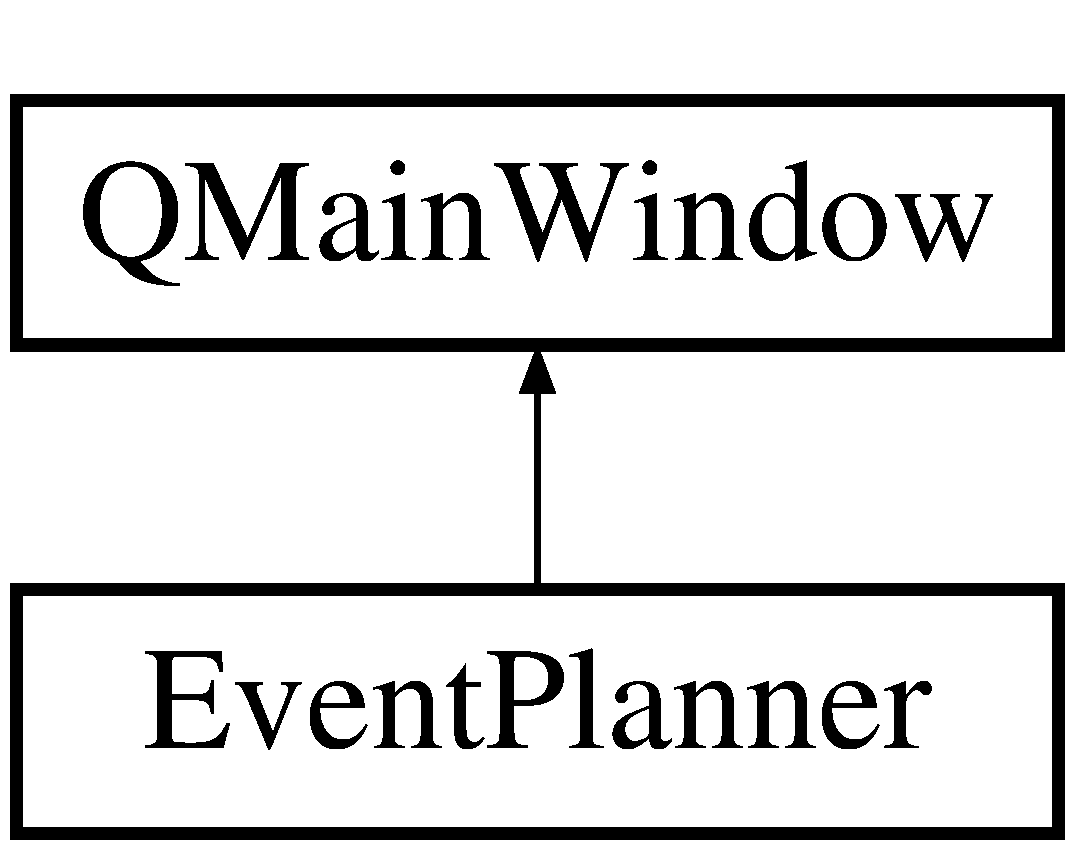
\includegraphics[height=2.000000cm]{class_event_planner}
\end{center}
\end{figure}
\subsection*{Signals}
\begin{DoxyCompactItemize}
\item 
void \hyperlink{class_event_planner_ac29d7162ba23478a3ca83d9a3451317e}{Adding\+Modeshow} ()
\begin{DoxyCompactList}\small\item\em Adding\+Modeshow. \end{DoxyCompactList}\item 
void \hyperlink{class_event_planner_a11d013b57831e685d134d824db883ad3}{Addingn\+Modequit} ()
\begin{DoxyCompactList}\small\item\em Addingn\+Modequit. \end{DoxyCompactList}\item 
void \hyperlink{class_event_planner_ae781e84143069d552b60b7856e7b0ad6}{Admin\+Modeshow} ()
\begin{DoxyCompactList}\small\item\em Admin\+Modeshow. \end{DoxyCompactList}\item 
void \hyperlink{class_event_planner_ab721a944eda1470ebb158bc815cc8734}{Admin\+Modequit} ()
\begin{DoxyCompactList}\small\item\em Admin\+Modequit. \end{DoxyCompactList}\item 
void \hyperlink{class_event_planner_a3c7b9e879f05ecb64f1d893084b1101c}{Logout} ()
\begin{DoxyCompactList}\small\item\em Logout. \end{DoxyCompactList}\end{DoxyCompactItemize}
\subsection*{Public Member Functions}
\begin{DoxyCompactItemize}
\item 
\hyperlink{class_event_planner_ae8b0e5c382c777476a003e3c099d5e38}{Event\+Planner} (Q\+Widget $\ast$parent=0)
\begin{DoxyCompactList}\small\item\em \hyperlink{class_event_planner}{Event\+Planner}. \end{DoxyCompactList}\item 
\hyperlink{class_event_planner_a0963c57038db491e25e7562a7701ae28}{$\sim$\+Event\+Planner} ()
\item 
void \hyperlink{class_event_planner_a2453c0478a2c0f60575e553dbea57f1e}{set\+Picture} ()
\begin{DoxyCompactList}\small\item\em set\+Picture \end{DoxyCompactList}\end{DoxyCompactItemize}


\subsection{Detailed Description}
The \hyperlink{class_event_planner}{Event\+Planner} class. 

Main menu window with options to either go to \hyperlink{class_event_admin_mode}{Event\+Admin\+Mode} or \hyperlink{class_adding_mode}{Adding\+Mode} 

\subsection{Constructor \& Destructor Documentation}
\mbox{\Hypertarget{class_event_planner_ae8b0e5c382c777476a003e3c099d5e38}\label{class_event_planner_ae8b0e5c382c777476a003e3c099d5e38}} 
\index{Event\+Planner@{Event\+Planner}!Event\+Planner@{Event\+Planner}}
\index{Event\+Planner@{Event\+Planner}!Event\+Planner@{Event\+Planner}}
\subsubsection{\texorpdfstring{Event\+Planner()}{EventPlanner()}}
{\footnotesize\ttfamily Event\+Planner\+::\+Event\+Planner (\begin{DoxyParamCaption}\item[{Q\+Widget $\ast$}]{parent = {\ttfamily 0} }\end{DoxyParamCaption})\hspace{0.3cm}{\ttfamily [explicit]}}



\hyperlink{class_event_planner}{Event\+Planner}. 

Construtor for menu window of main page. 
\begin{DoxyParams}{Parameters}
{\em parent} & \\
\hline
\end{DoxyParams}
\mbox{\Hypertarget{class_event_planner_a0963c57038db491e25e7562a7701ae28}\label{class_event_planner_a0963c57038db491e25e7562a7701ae28}} 
\index{Event\+Planner@{Event\+Planner}!````~Event\+Planner@{$\sim$\+Event\+Planner}}
\index{````~Event\+Planner@{$\sim$\+Event\+Planner}!Event\+Planner@{Event\+Planner}}
\subsubsection{\texorpdfstring{$\sim$\+Event\+Planner()}{~EventPlanner()}}
{\footnotesize\ttfamily Event\+Planner\+::$\sim$\+Event\+Planner (\begin{DoxyParamCaption}{ }\end{DoxyParamCaption})}



\subsection{Member Function Documentation}
\mbox{\Hypertarget{class_event_planner_ac29d7162ba23478a3ca83d9a3451317e}\label{class_event_planner_ac29d7162ba23478a3ca83d9a3451317e}} 
\index{Event\+Planner@{Event\+Planner}!Adding\+Modeshow@{Adding\+Modeshow}}
\index{Adding\+Modeshow@{Adding\+Modeshow}!Event\+Planner@{Event\+Planner}}
\subsubsection{\texorpdfstring{Adding\+Modeshow}{AddingModeshow}}
{\footnotesize\ttfamily void Event\+Planner\+::\+Adding\+Modeshow (\begin{DoxyParamCaption}{ }\end{DoxyParamCaption})\hspace{0.3cm}{\ttfamily [signal]}}



Adding\+Modeshow. 

Signal to switch to Adding Mode for adding availablity \mbox{\Hypertarget{class_event_planner_a11d013b57831e685d134d824db883ad3}\label{class_event_planner_a11d013b57831e685d134d824db883ad3}} 
\index{Event\+Planner@{Event\+Planner}!Addingn\+Modequit@{Addingn\+Modequit}}
\index{Addingn\+Modequit@{Addingn\+Modequit}!Event\+Planner@{Event\+Planner}}
\subsubsection{\texorpdfstring{Addingn\+Modequit}{AddingnModequit}}
{\footnotesize\ttfamily void Event\+Planner\+::\+Addingn\+Modequit (\begin{DoxyParamCaption}{ }\end{DoxyParamCaption})\hspace{0.3cm}{\ttfamily [signal]}}



Addingn\+Modequit. 

Signal that Addinf Mode was left \mbox{\Hypertarget{class_event_planner_ab721a944eda1470ebb158bc815cc8734}\label{class_event_planner_ab721a944eda1470ebb158bc815cc8734}} 
\index{Event\+Planner@{Event\+Planner}!Admin\+Modequit@{Admin\+Modequit}}
\index{Admin\+Modequit@{Admin\+Modequit}!Event\+Planner@{Event\+Planner}}
\subsubsection{\texorpdfstring{Admin\+Modequit}{AdminModequit}}
{\footnotesize\ttfamily void Event\+Planner\+::\+Admin\+Modequit (\begin{DoxyParamCaption}{ }\end{DoxyParamCaption})\hspace{0.3cm}{\ttfamily [signal]}}



Admin\+Modequit. 

Signal to say that Admin mode was exitted \mbox{\Hypertarget{class_event_planner_ae781e84143069d552b60b7856e7b0ad6}\label{class_event_planner_ae781e84143069d552b60b7856e7b0ad6}} 
\index{Event\+Planner@{Event\+Planner}!Admin\+Modeshow@{Admin\+Modeshow}}
\index{Admin\+Modeshow@{Admin\+Modeshow}!Event\+Planner@{Event\+Planner}}
\subsubsection{\texorpdfstring{Admin\+Modeshow}{AdminModeshow}}
{\footnotesize\ttfamily void Event\+Planner\+::\+Admin\+Modeshow (\begin{DoxyParamCaption}{ }\end{DoxyParamCaption})\hspace{0.3cm}{\ttfamily [signal]}}



Admin\+Modeshow. 

Signal to show Admin mode for creating events \mbox{\Hypertarget{class_event_planner_a3c7b9e879f05ecb64f1d893084b1101c}\label{class_event_planner_a3c7b9e879f05ecb64f1d893084b1101c}} 
\index{Event\+Planner@{Event\+Planner}!Logout@{Logout}}
\index{Logout@{Logout}!Event\+Planner@{Event\+Planner}}
\subsubsection{\texorpdfstring{Logout}{Logout}}
{\footnotesize\ttfamily void Event\+Planner\+::\+Logout (\begin{DoxyParamCaption}{ }\end{DoxyParamCaption})\hspace{0.3cm}{\ttfamily [signal]}}



Logout. 

Signal to return to Login Page \mbox{\Hypertarget{class_event_planner_a2453c0478a2c0f60575e553dbea57f1e}\label{class_event_planner_a2453c0478a2c0f60575e553dbea57f1e}} 
\index{Event\+Planner@{Event\+Planner}!set\+Picture@{set\+Picture}}
\index{set\+Picture@{set\+Picture}!Event\+Planner@{Event\+Planner}}
\subsubsection{\texorpdfstring{set\+Picture()}{setPicture()}}
{\footnotesize\ttfamily void Event\+Planner\+::set\+Picture (\begin{DoxyParamCaption}{ }\end{DoxyParamCaption})}



set\+Picture 

Adds picture to menu screen. 

The documentation for this class was generated from the following files\+:\begin{DoxyCompactItemize}
\item 
\hyperlink{eventplanner_8h}{eventplanner.\+h}\item 
\hyperlink{eventplanner_8cpp}{eventplanner.\+cpp}\end{DoxyCompactItemize}

\hypertarget{classhelpermethods}{}\section{helpermethods Class Reference}
\label{classhelpermethods}\index{helpermethods@{helpermethods}}


{\ttfamily \#include $<$helpermethods.\+h$>$}

\subsection*{Static Public Member Functions}
\begin{DoxyCompactItemize}
\item 
static Q\+String \hyperlink{classhelpermethods_a5357a7fde87ac02fce1e8ed64aa53648}{to\+Time} (int slot, bool format)
\begin{DoxyCompactList}\small\item\em to\+Time Will give specific time for given timeslot int e.\+g. 12$\vert$24h\+: 27 = 1\+:30pm$\vert$13\+:30 \end{DoxyCompactList}\item 
static Q\+String \hyperlink{classhelpermethods_a3ab55da6e3e7558936e9881f30465e75}{to\+Time\+Slot} (int timeslot, bool format)
\begin{DoxyCompactList}\small\item\em to\+Time\+Slot Will utilize to\+Time to create 30min timeslot string e.\+g. Timeslot-\/\+Timeslot+1\+: 27 = 1\+:30pm-\/2\+:00pm$\vert$13\+:30-\/14\+:00 \end{DoxyCompactList}\item 
static Q\+String \hyperlink{classhelpermethods_a8eb0fa4dbe1ac5465ba69976ed93b7e9}{get\+Time\+String} (Q\+List$<$ int $>$ timeslots, bool format)
\begin{DoxyCompactList}\small\item\em get\+Time\+String Returns a smarter timeslot string based on contiguous timeslots \end{DoxyCompactList}\item 
static Q\+String \hyperlink{classhelpermethods_aa6324bf2fa835db5e8baacc6500e0447}{stringify\+Timeslot\+Ints} (Q\+List$<$ int $>$ timeslots)
\begin{DoxyCompactList}\small\item\em stringify\+Timeslot\+Ints Inverse function of listify\+Timeslot\+Ints \end{DoxyCompactList}\item 
static Q\+List$<$ int $>$ \hyperlink{classhelpermethods_ab2c39e2fbd1d97104b57f8f5cbf2c3ab}{listify\+Timeslot\+Ints} (Q\+String timeslot\+String)
\begin{DoxyCompactList}\small\item\em listify\+Timeslot\+Ints Inverse function of stringify\+Timeslot\+Ints \end{DoxyCompactList}\item 
static bool \hyperlink{classhelpermethods_a78e0af34a4ee72796f2e1ea3504bf678}{compare\+Dates} (Q\+String date1, Q\+String date2)
\begin{DoxyCompactList}\small\item\em compare\+Dates Essentially a $<$ function for dates of format \char`\"{}\+M\+M-\/\+D\+D-\/\+Y\+Y\+Y\+Y\char`\"{} \end{DoxyCompactList}\end{DoxyCompactItemize}


\subsection{Member Function Documentation}
\mbox{\Hypertarget{classhelpermethods_a78e0af34a4ee72796f2e1ea3504bf678}\label{classhelpermethods_a78e0af34a4ee72796f2e1ea3504bf678}} 
\index{helpermethods@{helpermethods}!compare\+Dates@{compare\+Dates}}
\index{compare\+Dates@{compare\+Dates}!helpermethods@{helpermethods}}
\subsubsection{\texorpdfstring{compare\+Dates()}{compareDates()}}
{\footnotesize\ttfamily bool helpermethods\+::compare\+Dates (\begin{DoxyParamCaption}\item[{Q\+String}]{date1,  }\item[{Q\+String}]{date2 }\end{DoxyParamCaption})\hspace{0.3cm}{\ttfamily [static]}}



compare\+Dates Essentially a $<$ function for dates of format \char`\"{}\+M\+M-\/\+D\+D-\/\+Y\+Y\+Y\+Y\char`\"{} 


\begin{DoxyParams}{Parameters}
{\em date1} & \\
\hline
{\em date2} & \\
\hline
\end{DoxyParams}
\begin{DoxyReturn}{Returns}
True if date1 is prior to date2. False otherwise 
\end{DoxyReturn}
\mbox{\Hypertarget{classhelpermethods_a8eb0fa4dbe1ac5465ba69976ed93b7e9}\label{classhelpermethods_a8eb0fa4dbe1ac5465ba69976ed93b7e9}} 
\index{helpermethods@{helpermethods}!get\+Time\+String@{get\+Time\+String}}
\index{get\+Time\+String@{get\+Time\+String}!helpermethods@{helpermethods}}
\subsubsection{\texorpdfstring{get\+Time\+String()}{getTimeString()}}
{\footnotesize\ttfamily Q\+String helpermethods\+::get\+Time\+String (\begin{DoxyParamCaption}\item[{Q\+List$<$ int $>$}]{timeslots,  }\item[{bool}]{format }\end{DoxyParamCaption})\hspace{0.3cm}{\ttfamily [static]}}



get\+Time\+String Returns a smarter timeslot string based on contiguous timeslots 


\begin{DoxyParams}{Parameters}
{\em timeslots} & Will sort then utilize list of ints with range 0-\/47 \\
\hline
{\em format} & T\+R\+UE\+: 24h format $\vert$ F\+A\+L\+SE\+: 12h format \\
\hline
\end{DoxyParams}
\begin{DoxyReturn}{Returns}

\end{DoxyReturn}
\mbox{\Hypertarget{classhelpermethods_ab2c39e2fbd1d97104b57f8f5cbf2c3ab}\label{classhelpermethods_ab2c39e2fbd1d97104b57f8f5cbf2c3ab}} 
\index{helpermethods@{helpermethods}!listify\+Timeslot\+Ints@{listify\+Timeslot\+Ints}}
\index{listify\+Timeslot\+Ints@{listify\+Timeslot\+Ints}!helpermethods@{helpermethods}}
\subsubsection{\texorpdfstring{listify\+Timeslot\+Ints()}{listifyTimeslotInts()}}
{\footnotesize\ttfamily Q\+List$<$ int $>$ helpermethods\+::listify\+Timeslot\+Ints (\begin{DoxyParamCaption}\item[{Q\+String}]{timeslot\+String }\end{DoxyParamCaption})\hspace{0.3cm}{\ttfamily [static]}}



listify\+Timeslot\+Ints Inverse function of stringify\+Timeslot\+Ints 


\begin{DoxyParams}{Parameters}
{\em timeslot\+String} & e.\+g. \char`\"{}0,1,2,3,4\char`\"{} \\
\hline
\end{DoxyParams}
\begin{DoxyReturn}{Returns}
Q\+List of timeslots 
\end{DoxyReturn}
\mbox{\Hypertarget{classhelpermethods_aa6324bf2fa835db5e8baacc6500e0447}\label{classhelpermethods_aa6324bf2fa835db5e8baacc6500e0447}} 
\index{helpermethods@{helpermethods}!stringify\+Timeslot\+Ints@{stringify\+Timeslot\+Ints}}
\index{stringify\+Timeslot\+Ints@{stringify\+Timeslot\+Ints}!helpermethods@{helpermethods}}
\subsubsection{\texorpdfstring{stringify\+Timeslot\+Ints()}{stringifyTimeslotInts()}}
{\footnotesize\ttfamily Q\+String helpermethods\+::stringify\+Timeslot\+Ints (\begin{DoxyParamCaption}\item[{Q\+List$<$ int $>$}]{timeslots }\end{DoxyParamCaption})\hspace{0.3cm}{\ttfamily [static]}}



stringify\+Timeslot\+Ints Inverse function of listify\+Timeslot\+Ints 


\begin{DoxyParams}{Parameters}
{\em timeslots} & Q\+List$<$int$>$ \\
\hline
\end{DoxyParams}
\begin{DoxyReturn}{Returns}
Q\+String of timeslots e.\+g. \char`\"{}0,1,2,3,4\char`\"{} 
\end{DoxyReturn}
\mbox{\Hypertarget{classhelpermethods_a5357a7fde87ac02fce1e8ed64aa53648}\label{classhelpermethods_a5357a7fde87ac02fce1e8ed64aa53648}} 
\index{helpermethods@{helpermethods}!to\+Time@{to\+Time}}
\index{to\+Time@{to\+Time}!helpermethods@{helpermethods}}
\subsubsection{\texorpdfstring{to\+Time()}{toTime()}}
{\footnotesize\ttfamily Q\+String helpermethods\+::to\+Time (\begin{DoxyParamCaption}\item[{int}]{slot,  }\item[{bool}]{format }\end{DoxyParamCaption})\hspace{0.3cm}{\ttfamily [static]}}



to\+Time Will give specific time for given timeslot int e.\+g. 12$\vert$24h\+: 27 = 1\+:30pm$\vert$13\+:30 


\begin{DoxyParams}{Parameters}
{\em timeslot} & 0-\/47 \\
\hline
{\em format} & T\+R\+UE\+: 24h format $\vert$ F\+A\+L\+SE\+: 12h format \\
\hline
\end{DoxyParams}
\begin{DoxyReturn}{Returns}
Q\+String Time in 12h/24h format 
\end{DoxyReturn}
\mbox{\Hypertarget{classhelpermethods_a3ab55da6e3e7558936e9881f30465e75}\label{classhelpermethods_a3ab55da6e3e7558936e9881f30465e75}} 
\index{helpermethods@{helpermethods}!to\+Time\+Slot@{to\+Time\+Slot}}
\index{to\+Time\+Slot@{to\+Time\+Slot}!helpermethods@{helpermethods}}
\subsubsection{\texorpdfstring{to\+Time\+Slot()}{toTimeSlot()}}
{\footnotesize\ttfamily Q\+String helpermethods\+::to\+Time\+Slot (\begin{DoxyParamCaption}\item[{int}]{timeslot,  }\item[{bool}]{format }\end{DoxyParamCaption})\hspace{0.3cm}{\ttfamily [static]}}



to\+Time\+Slot Will utilize to\+Time to create 30min timeslot string e.\+g. Timeslot-\/\+Timeslot+1\+: 27 = 1\+:30pm-\/2\+:00pm$\vert$13\+:30-\/14\+:00 


\begin{DoxyParams}{Parameters}
{\em timeslot} & 0-\/47 \\
\hline
{\em format} & T\+R\+UE\+: 24h format $\vert$ F\+A\+L\+SE\+: 12h format \\
\hline
\end{DoxyParams}
\begin{DoxyReturn}{Returns}

\end{DoxyReturn}


The documentation for this class was generated from the following files\+:\begin{DoxyCompactItemize}
\item 
\hyperlink{helpermethods_8h}{helpermethods.\+h}\item 
\hyperlink{helpermethods_8cpp}{helpermethods.\+cpp}\end{DoxyCompactItemize}

\hypertarget{class_login_page}{}\section{Login\+Page Class Reference}
\label{class_login_page}\index{Login\+Page@{Login\+Page}}


The \hyperlink{class_login_page}{Login\+Page} class.  




{\ttfamily \#include $<$loginpage.\+h$>$}

Inheritance diagram for Login\+Page\+:\begin{figure}[H]
\begin{center}
\leavevmode
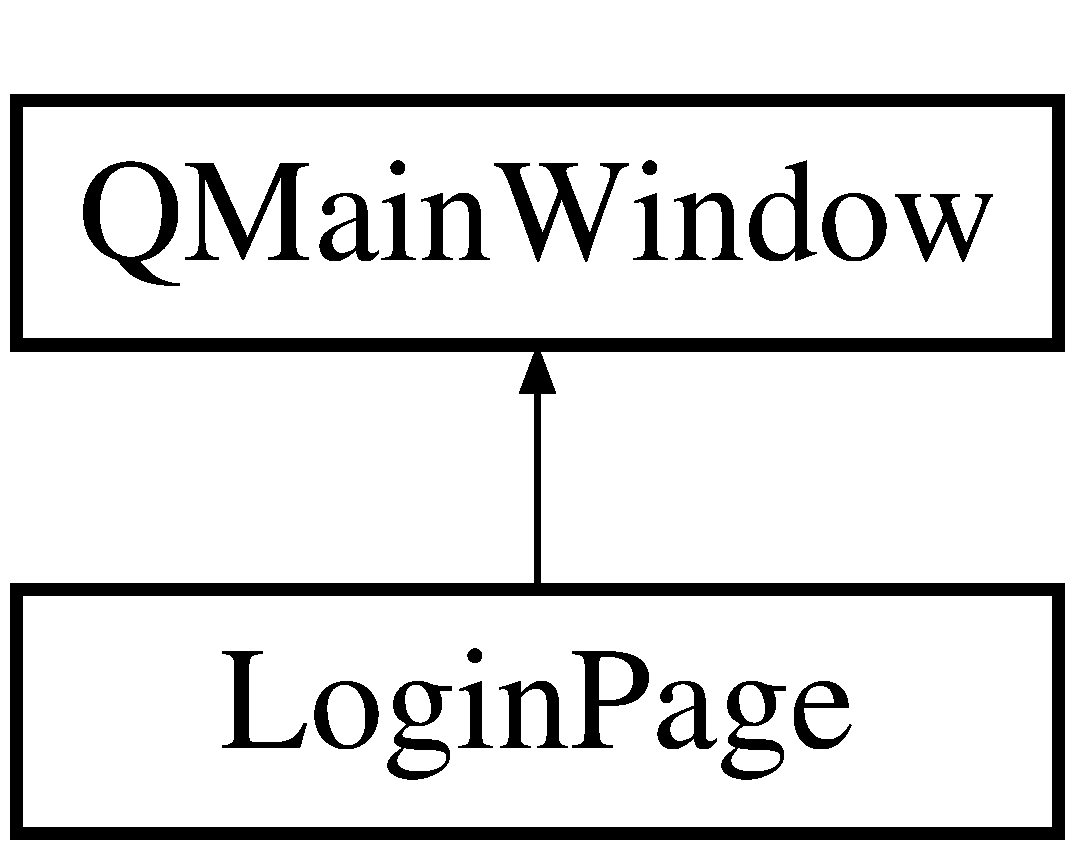
\includegraphics[height=2.000000cm]{class_login_page}
\end{center}
\end{figure}
\subsection*{Signals}
\begin{DoxyCompactItemize}
\item 
void \hyperlink{class_login_page_a7b74b87a3affb709ea585fb556a57271}{go\+To\+Event\+Planner} ()
\begin{DoxyCompactList}\small\item\em go\+To\+Event\+Planner \end{DoxyCompactList}\end{DoxyCompactItemize}
\subsection*{Public Member Functions}
\begin{DoxyCompactItemize}
\item 
\hyperlink{class_login_page_aabf302d725edb6a1a0e8cca53f9b3fbf}{Login\+Page} (\hyperlink{class_session}{Session} $\ast$session, Q\+Widget $\ast$parent=0)
\begin{DoxyCompactList}\small\item\em \hyperlink{class_login_page}{Login\+Page}. \end{DoxyCompactList}\item 
\hyperlink{class_login_page_ae3c843938f34258ac50eb89d30d31d8a}{$\sim$\+Login\+Page} ()
\end{DoxyCompactItemize}


\subsection{Detailed Description}
The \hyperlink{class_login_page}{Login\+Page} class. 

Class for buidling the Login Page 

\subsection{Constructor \& Destructor Documentation}
\mbox{\Hypertarget{class_login_page_aabf302d725edb6a1a0e8cca53f9b3fbf}\label{class_login_page_aabf302d725edb6a1a0e8cca53f9b3fbf}} 
\index{Login\+Page@{Login\+Page}!Login\+Page@{Login\+Page}}
\index{Login\+Page@{Login\+Page}!Login\+Page@{Login\+Page}}
\subsubsection{\texorpdfstring{Login\+Page()}{LoginPage()}}
{\footnotesize\ttfamily Login\+Page\+::\+Login\+Page (\begin{DoxyParamCaption}\item[{\hyperlink{class_session}{Session} $\ast$}]{session,  }\item[{Q\+Widget $\ast$}]{parent = {\ttfamily 0} }\end{DoxyParamCaption})\hspace{0.3cm}{\ttfamily [explicit]}}



\hyperlink{class_login_page}{Login\+Page}. 

Constructor for \hyperlink{class_login_page}{Login\+Page} class 
\begin{DoxyParams}{Parameters}
{\em session} & \\
\hline
{\em parent} & \\
\hline
\end{DoxyParams}
\mbox{\Hypertarget{class_login_page_ae3c843938f34258ac50eb89d30d31d8a}\label{class_login_page_ae3c843938f34258ac50eb89d30d31d8a}} 
\index{Login\+Page@{Login\+Page}!````~Login\+Page@{$\sim$\+Login\+Page}}
\index{````~Login\+Page@{$\sim$\+Login\+Page}!Login\+Page@{Login\+Page}}
\subsubsection{\texorpdfstring{$\sim$\+Login\+Page()}{~LoginPage()}}
{\footnotesize\ttfamily Login\+Page\+::$\sim$\+Login\+Page (\begin{DoxyParamCaption}{ }\end{DoxyParamCaption})}



\subsection{Member Function Documentation}
\mbox{\Hypertarget{class_login_page_a7b74b87a3affb709ea585fb556a57271}\label{class_login_page_a7b74b87a3affb709ea585fb556a57271}} 
\index{Login\+Page@{Login\+Page}!go\+To\+Event\+Planner@{go\+To\+Event\+Planner}}
\index{go\+To\+Event\+Planner@{go\+To\+Event\+Planner}!Login\+Page@{Login\+Page}}
\subsubsection{\texorpdfstring{go\+To\+Event\+Planner}{goToEventPlanner}}
{\footnotesize\ttfamily void Login\+Page\+::go\+To\+Event\+Planner (\begin{DoxyParamCaption}{ }\end{DoxyParamCaption})\hspace{0.3cm}{\ttfamily [signal]}}



go\+To\+Event\+Planner 

Signal for transitiong to the \hyperlink{class_event}{Event} Planner page. 

The documentation for this class was generated from the following files\+:\begin{DoxyCompactItemize}
\item 
\hyperlink{loginpage_8h}{loginpage.\+h}\item 
\hyperlink{loginpage_8cpp}{loginpage.\+cpp}\end{DoxyCompactItemize}

\hypertarget{class_session}{}\section{Session Class Reference}
\label{class_session}\index{Session@{Session}}


The \hyperlink{class_session}{Session} class.  




{\ttfamily \#include $<$session.\+h$>$}

\subsection*{Public Member Functions}
\begin{DoxyCompactItemize}
\item 
\hyperlink{class_session_ad92ef09b872c9227e38a6efdd4d8a837}{Session} ()
\begin{DoxyCompactList}\small\item\em \hyperlink{class_session}{Session}. \end{DoxyCompactList}\item 
\hyperlink{class_session_a0a7362dd58b94a67af892eb2cda1082a}{Session} (Q\+String user)
\begin{DoxyCompactList}\small\item\em \hyperlink{class_session}{Session}. \end{DoxyCompactList}\item 
\hyperlink{class_session_a8753bb9dee966b7d39abc9b7237cd665}{$\sim$\+Session} ()
\item 
void \hyperlink{class_session_a195911688579c457cf7e71c29ded7489}{add\+Event} (Q\+String owner, Q\+String event\+Name, int event\+ID, Q\+String\+List event\+Days, Q\+String\+List event\+Tasks, Q\+List$<$ int $>$ time\+Slots, \hyperlink{classattendee}{attendee} $\ast$att)
\begin{DoxyCompactList}\small\item\em add\+Event \end{DoxyCompactList}\item 
bool \hyperlink{class_session_aff9fd19eb09a0ac22d3e2c2615f9f9e9}{read\+Events\+From\+File} ()
\begin{DoxyCompactList}\small\item\em read\+Events\+From\+File \end{DoxyCompactList}\item 
bool \hyperlink{class_session_af095af8449dd10f6fdf3db6d530e109e}{save\+Events\+To\+File} ()
\begin{DoxyCompactList}\small\item\em save\+Events\+To\+File \end{DoxyCompactList}\item 
Q\+String \hyperlink{class_session_a09e51bffb8d4657efcb8ccf47be3192d}{get\+User} () const
\begin{DoxyCompactList}\small\item\em get\+User \end{DoxyCompactList}\item 
void \hyperlink{class_session_a3e4500bdcf80458ae14dde3eb413adb8}{set\+User} (Q\+String user)
\begin{DoxyCompactList}\small\item\em set\+User \end{DoxyCompactList}\item 
std\+::list$<$ \hyperlink{class_event}{Event} $\ast$ $>$ \& \hyperlink{class_session_a9712e356f0d5c3efdaed996ddc063738}{get\+Events} ()
\begin{DoxyCompactList}\small\item\em get\+Events \end{DoxyCompactList}\item 
int \hyperlink{class_session_aa6766de9b237384f6eff9ccbdfd8bde9}{number\+Of\+Events} () const
\begin{DoxyCompactList}\small\item\em number\+Of\+Events \end{DoxyCompactList}\end{DoxyCompactItemize}


\subsection{Detailed Description}
The \hyperlink{class_session}{Session} class. 

The session object is used to handle reading and writing events to file for storage as well as stroing events in memory while program is running. 

\subsection{Constructor \& Destructor Documentation}
\mbox{\Hypertarget{class_session_ad92ef09b872c9227e38a6efdd4d8a837}\label{class_session_ad92ef09b872c9227e38a6efdd4d8a837}} 
\index{Session@{Session}!Session@{Session}}
\index{Session@{Session}!Session@{Session}}
\subsubsection{\texorpdfstring{Session()}{Session()}\hspace{0.1cm}{\footnotesize\ttfamily [1/2]}}
{\footnotesize\ttfamily Session\+::\+Session (\begin{DoxyParamCaption}{ }\end{DoxyParamCaption})}



\hyperlink{class_session}{Session}. 

Default constructor. All initializations are set to default. \mbox{\Hypertarget{class_session_a0a7362dd58b94a67af892eb2cda1082a}\label{class_session_a0a7362dd58b94a67af892eb2cda1082a}} 
\index{Session@{Session}!Session@{Session}}
\index{Session@{Session}!Session@{Session}}
\subsubsection{\texorpdfstring{Session()}{Session()}\hspace{0.1cm}{\footnotesize\ttfamily [2/2]}}
{\footnotesize\ttfamily Session\+::\+Session (\begin{DoxyParamCaption}\item[{Q\+String}]{user }\end{DoxyParamCaption})}



\hyperlink{class_session}{Session}. 

Constructor where private memebr variable Q\+String user is set to the passed argument. 
\begin{DoxyParams}{Parameters}
{\em user} & \\
\hline
\end{DoxyParams}
\mbox{\Hypertarget{class_session_a8753bb9dee966b7d39abc9b7237cd665}\label{class_session_a8753bb9dee966b7d39abc9b7237cd665}} 
\index{Session@{Session}!````~Session@{$\sim$\+Session}}
\index{````~Session@{$\sim$\+Session}!Session@{Session}}
\subsubsection{\texorpdfstring{$\sim$\+Session()}{~Session()}}
{\footnotesize\ttfamily Session\+::$\sim$\+Session (\begin{DoxyParamCaption}{ }\end{DoxyParamCaption})}



\subsection{Member Function Documentation}
\mbox{\Hypertarget{class_session_a195911688579c457cf7e71c29ded7489}\label{class_session_a195911688579c457cf7e71c29ded7489}} 
\index{Session@{Session}!add\+Event@{add\+Event}}
\index{add\+Event@{add\+Event}!Session@{Session}}
\subsubsection{\texorpdfstring{add\+Event()}{addEvent()}}
{\footnotesize\ttfamily void Session\+::add\+Event (\begin{DoxyParamCaption}\item[{Q\+String}]{owner,  }\item[{Q\+String}]{event\+Name,  }\item[{int}]{event\+ID,  }\item[{Q\+String\+List}]{event\+Days,  }\item[{Q\+String\+List}]{event\+Tasks,  }\item[{Q\+List$<$ int $>$}]{time\+Slots,  }\item[{\hyperlink{classattendee}{attendee} $\ast$}]{att }\end{DoxyParamCaption})}



add\+Event 

Creates a new \hyperlink{class_event}{Event} using the passed arguments and pushes it to the end of private memeber variable td\+::list$<$\+Event$\ast$$>$ events. 
\begin{DoxyParams}{Parameters}
{\em owner} & \\
\hline
{\em event\+Name} & \\
\hline
{\em month} & \\
\hline
{\em day} & \\
\hline
{\em year} & \\
\hline
{\em time\+Slots} & \\
\hline
\end{DoxyParams}
\mbox{\Hypertarget{class_session_a9712e356f0d5c3efdaed996ddc063738}\label{class_session_a9712e356f0d5c3efdaed996ddc063738}} 
\index{Session@{Session}!get\+Events@{get\+Events}}
\index{get\+Events@{get\+Events}!Session@{Session}}
\subsubsection{\texorpdfstring{get\+Events()}{getEvents()}}
{\footnotesize\ttfamily std\+::list$<$ \hyperlink{class_event}{Event} $\ast$ $>$ \& Session\+::get\+Events (\begin{DoxyParamCaption}{ }\end{DoxyParamCaption})}



get\+Events 

Returns the private member variable std\+::list$<$\+Event$\ast$$>$ events. This is a list of \hyperlink{class_event}{Event} pointers of all Events avaivalbe in the \hyperlink{class_session}{Session}. \begin{DoxyReturn}{Returns}
std\+::list$<$\+Event$\ast$$>$ 
\end{DoxyReturn}
\mbox{\Hypertarget{class_session_a09e51bffb8d4657efcb8ccf47be3192d}\label{class_session_a09e51bffb8d4657efcb8ccf47be3192d}} 
\index{Session@{Session}!get\+User@{get\+User}}
\index{get\+User@{get\+User}!Session@{Session}}
\subsubsection{\texorpdfstring{get\+User()}{getUser()}}
{\footnotesize\ttfamily Q\+String Session\+::get\+User (\begin{DoxyParamCaption}{ }\end{DoxyParamCaption}) const}



get\+User 

Returns the private member Q\+String user. \begin{DoxyReturn}{Returns}
Q\+String 
\end{DoxyReturn}
\mbox{\Hypertarget{class_session_aa6766de9b237384f6eff9ccbdfd8bde9}\label{class_session_aa6766de9b237384f6eff9ccbdfd8bde9}} 
\index{Session@{Session}!number\+Of\+Events@{number\+Of\+Events}}
\index{number\+Of\+Events@{number\+Of\+Events}!Session@{Session}}
\subsubsection{\texorpdfstring{number\+Of\+Events()}{numberOfEvents()}}
{\footnotesize\ttfamily int Session\+::number\+Of\+Events (\begin{DoxyParamCaption}{ }\end{DoxyParamCaption}) const}



number\+Of\+Events 

Returns the size of std\+::list$<$\+Event$\ast$$>$ events. \begin{DoxyReturn}{Returns}
int 
\end{DoxyReturn}
\mbox{\Hypertarget{class_session_aff9fd19eb09a0ac22d3e2c2615f9f9e9}\label{class_session_aff9fd19eb09a0ac22d3e2c2615f9f9e9}} 
\index{Session@{Session}!read\+Events\+From\+File@{read\+Events\+From\+File}}
\index{read\+Events\+From\+File@{read\+Events\+From\+File}!Session@{Session}}
\subsubsection{\texorpdfstring{read\+Events\+From\+File()}{readEventsFromFile()}}
{\footnotesize\ttfamily bool Session\+::read\+Events\+From\+File (\begin{DoxyParamCaption}{ }\end{DoxyParamCaption})}



read\+Events\+From\+File 

Reads in contents of Event\+Data.\+txt and parses for \hyperlink{class_event}{Event} objects. Events objects are the pushed into std\+::list$<$\+Event$\ast$$>$ events. \begin{DoxyReturn}{Returns}
True if file succesfully parsed. False otherwise. 
\end{DoxyReturn}
\mbox{\Hypertarget{class_session_af095af8449dd10f6fdf3db6d530e109e}\label{class_session_af095af8449dd10f6fdf3db6d530e109e}} 
\index{Session@{Session}!save\+Events\+To\+File@{save\+Events\+To\+File}}
\index{save\+Events\+To\+File@{save\+Events\+To\+File}!Session@{Session}}
\subsubsection{\texorpdfstring{save\+Events\+To\+File()}{saveEventsToFile()}}
{\footnotesize\ttfamily bool Session\+::save\+Events\+To\+File (\begin{DoxyParamCaption}{ }\end{DoxyParamCaption})}



save\+Events\+To\+File 

Writes formatted contents of std\+::list$<$\+Event$\ast$$>$ events to file Event\+Data.\+txt. \begin{DoxyReturn}{Returns}
True if file succesfully saved. False otherwise. 
\end{DoxyReturn}
\mbox{\Hypertarget{class_session_a3e4500bdcf80458ae14dde3eb413adb8}\label{class_session_a3e4500bdcf80458ae14dde3eb413adb8}} 
\index{Session@{Session}!set\+User@{set\+User}}
\index{set\+User@{set\+User}!Session@{Session}}
\subsubsection{\texorpdfstring{set\+User()}{setUser()}}
{\footnotesize\ttfamily void Session\+::set\+User (\begin{DoxyParamCaption}\item[{Q\+String}]{user }\end{DoxyParamCaption})}



set\+User 

Sets the private member variable Q\+String user to the passed argument. 
\begin{DoxyParams}{Parameters}
{\em user} & \\
\hline
\end{DoxyParams}


The documentation for this class was generated from the following files\+:\begin{DoxyCompactItemize}
\item 
\hyperlink{session_8h}{session.\+h}\item 
\hyperlink{session_8cpp}{session.\+cpp}\end{DoxyCompactItemize}

\chapter{File Documentation}
\hypertarget{addingmode_8cpp}{}\section{addingmode.\+cpp File Reference}
\label{addingmode_8cpp}\index{addingmode.\+cpp@{addingmode.\+cpp}}
{\ttfamily \#include \char`\"{}addingmode.\+h\char`\"{}}\newline
{\ttfamily \#include \char`\"{}ui\+\_\+addingmode.\+h\char`\"{}}\newline
{\ttfamily \#include \char`\"{}eventplanner.\+h\char`\"{}}\newline
{\ttfamily \#include $<$Q\+String$>$}\newline
{\ttfamily \#include $<$Q\+List$>$}\newline

\hypertarget{addingmode_8h}{}\section{addingmode.\+h File Reference}
\label{addingmode_8h}\index{addingmode.\+h@{addingmode.\+h}}
{\ttfamily \#include $<$Q\+Main\+Window$>$}\newline
{\ttfamily \#include \char`\"{}session.\+h\char`\"{}}\newline
{\ttfamily \#include \char`\"{}event.\+h\char`\"{}}\newline
{\ttfamily \#include \char`\"{}helpermethods.\+h\char`\"{}}\newline
{\ttfamily \#include \char`\"{}attendee.\+h\char`\"{}}\newline
{\ttfamily \#include $<$list$>$}\newline
{\ttfamily \#include $<$Q\+Debug$>$}\newline
\subsection*{Classes}
\begin{DoxyCompactItemize}
\item 
class \hyperlink{class_adding_mode}{Adding\+Mode}
\begin{DoxyCompactList}\small\item\em The \hyperlink{class_adding_mode}{Adding\+Mode} class. \end{DoxyCompactList}\end{DoxyCompactItemize}
\subsection*{Namespaces}
\begin{DoxyCompactItemize}
\item 
 \hyperlink{namespace_ui}{Ui}
\end{DoxyCompactItemize}

\hypertarget{attendee_8cpp}{}\section{attendee.\+cpp File Reference}
\label{attendee_8cpp}\index{attendee.\+cpp@{attendee.\+cpp}}
{\ttfamily \#include \char`\"{}attendee.\+h\char`\"{}}\newline

\hypertarget{attendee_8h}{}\section{attendee.\+h File Reference}
\label{attendee_8h}\index{attendee.\+h@{attendee.\+h}}
{\ttfamily \#include $<$Q\+String$>$}\newline
{\ttfamily \#include $<$Q\+List$>$}\newline
\subsection*{Classes}
\begin{DoxyCompactItemize}
\item 
class \hyperlink{classattendee}{attendee}
\end{DoxyCompactItemize}

\hypertarget{event_8cpp}{}\section{event.\+cpp File Reference}
\label{event_8cpp}\index{event.\+cpp@{event.\+cpp}}
{\ttfamily \#include \char`\"{}event.\+h\char`\"{}}\newline
{\ttfamily \#include $<$list$>$}\newline

\hypertarget{event_8h}{}\section{event.\+h File Reference}
\label{event_8h}\index{event.\+h@{event.\+h}}
{\ttfamily \#include \char`\"{}attendee.\+h\char`\"{}}\newline
{\ttfamily \#include $<$list$>$}\newline
{\ttfamily \#include $<$Q\+String$>$}\newline
{\ttfamily \#include $<$Q\+String\+List$>$}\newline
\subsection*{Classes}
\begin{DoxyCompactItemize}
\item 
class \hyperlink{class_event}{Event}
\begin{DoxyCompactList}\small\item\em The \hyperlink{class_event}{Event} class. \end{DoxyCompactList}\end{DoxyCompactItemize}

\hypertarget{eventadminmode_8cpp}{}\section{eventadminmode.\+cpp File Reference}
\label{eventadminmode_8cpp}\index{eventadminmode.\+cpp@{eventadminmode.\+cpp}}
{\ttfamily \#include \char`\"{}eventadminmode.\+h\char`\"{}}\newline
{\ttfamily \#include \char`\"{}ui\+\_\+eventadminmode.\+h\char`\"{}}\newline

\hypertarget{eventadminmode_8h}{}\section{eventadminmode.\+h File Reference}
\label{eventadminmode_8h}\index{eventadminmode.\+h@{eventadminmode.\+h}}
{\ttfamily \#include $<$Q\+Main\+Window$>$}\newline
{\ttfamily \#include $<$Q\+Debug$>$}\newline
{\ttfamily \#include \char`\"{}session.\+h\char`\"{}}\newline
{\ttfamily \#include \char`\"{}helpermethods.\+h\char`\"{}}\newline
{\ttfamily \#include $<$eventplanner.\+h$>$}\newline
{\ttfamily \#include $<$Q\+Message\+Box$>$}\newline
{\ttfamily \#include $<$Q\+Push\+Button$>$}\newline
{\ttfamily \#include $<$Q\+Tool\+Button$>$}\newline
{\ttfamily \#include $<$Q\+Pixmap$>$}\newline
{\ttfamily \#include $<$Q\+Icon$>$}\newline
{\ttfamily \#include $<$ctime$>$}\newline
{\ttfamily \#include $<$Q\+String$>$}\newline
{\ttfamily \#include $<$Qpen$>$}\newline
\subsection*{Classes}
\begin{DoxyCompactItemize}
\item 
class \hyperlink{class_event_admin_mode}{Event\+Admin\+Mode}
\begin{DoxyCompactList}\small\item\em The \hyperlink{class_event_admin_mode}{Event\+Admin\+Mode} class. \end{DoxyCompactList}\end{DoxyCompactItemize}
\subsection*{Namespaces}
\begin{DoxyCompactItemize}
\item 
 \hyperlink{namespace_ui}{Ui}
\end{DoxyCompactItemize}

\hypertarget{eventplanner_8cpp}{}\section{eventplanner.\+cpp File Reference}
\label{eventplanner_8cpp}\index{eventplanner.\+cpp@{eventplanner.\+cpp}}
{\ttfamily \#include \char`\"{}eventplanner.\+h\char`\"{}}\newline
{\ttfamily \#include \char`\"{}ui\+\_\+eventplanner.\+h\char`\"{}}\newline

\hypertarget{eventplanner_8h}{}\section{eventplanner.\+h File Reference}
\label{eventplanner_8h}\index{eventplanner.\+h@{eventplanner.\+h}}
{\ttfamily \#include $<$Q\+Main\+Window$>$}\newline
{\ttfamily \#include $<$Q\+Message\+Box$>$}\newline
{\ttfamily \#include $<$Q\+Pixmap$>$}\newline
\subsection*{Classes}
\begin{DoxyCompactItemize}
\item 
class \hyperlink{class_event_planner}{Event\+Planner}
\begin{DoxyCompactList}\small\item\em The \hyperlink{class_event_planner}{Event\+Planner} class. \end{DoxyCompactList}\end{DoxyCompactItemize}
\subsection*{Namespaces}
\begin{DoxyCompactItemize}
\item 
 \hyperlink{namespace_ui}{Ui}
\end{DoxyCompactItemize}

\hypertarget{helpermethods_8cpp}{}\section{helpermethods.\+cpp File Reference}
\label{helpermethods_8cpp}\index{helpermethods.\+cpp@{helpermethods.\+cpp}}
{\ttfamily \#include \char`\"{}helpermethods.\+h\char`\"{}}\newline

\hypertarget{helpermethods_8h}{}\section{helpermethods.\+h File Reference}
\label{helpermethods_8h}\index{helpermethods.\+h@{helpermethods.\+h}}
{\ttfamily \#include $<$Q\+List$>$}\newline
{\ttfamily \#include $<$Q\+String$>$}\newline
{\ttfamily \#include $<$Q\+Variant$>$}\newline
\subsection*{Classes}
\begin{DoxyCompactItemize}
\item 
class \hyperlink{classhelpermethods}{helpermethods}
\end{DoxyCompactItemize}

\hypertarget{loginpage_8cpp}{}\section{loginpage.\+cpp File Reference}
\label{loginpage_8cpp}\index{loginpage.\+cpp@{loginpage.\+cpp}}
{\ttfamily \#include \char`\"{}loginpage.\+h\char`\"{}}\newline
{\ttfamily \#include \char`\"{}ui\+\_\+loginpage.\+h\char`\"{}}\newline
{\ttfamily \#include $<$Q\+Message\+Box$>$}\newline

\hypertarget{loginpage_8h}{}\section{loginpage.\+h File Reference}
\label{loginpage_8h}\index{loginpage.\+h@{loginpage.\+h}}
{\ttfamily \#include \char`\"{}session.\+h\char`\"{}}\newline
{\ttfamily \#include $<$Q\+Main\+Window$>$}\newline
\subsection*{Classes}
\begin{DoxyCompactItemize}
\item 
class \hyperlink{class_login_page}{Login\+Page}
\begin{DoxyCompactList}\small\item\em The \hyperlink{class_login_page}{Login\+Page} class. \end{DoxyCompactList}\end{DoxyCompactItemize}
\subsection*{Namespaces}
\begin{DoxyCompactItemize}
\item 
 \hyperlink{namespace_ui}{Ui}
\end{DoxyCompactItemize}

\hypertarget{main_8cpp}{}\section{main.\+cpp File Reference}
\label{main_8cpp}\index{main.\+cpp@{main.\+cpp}}
{\ttfamily \#include \char`\"{}eventplanner.\+h\char`\"{}}\newline
{\ttfamily \#include \char`\"{}eventadminmode.\+h\char`\"{}}\newline
{\ttfamily \#include \char`\"{}addingmode.\+h\char`\"{}}\newline
{\ttfamily \#include \char`\"{}session.\+h\char`\"{}}\newline
{\ttfamily \#include \char`\"{}loginpage.\+h\char`\"{}}\newline
{\ttfamily \#include $<$Q\+Application$>$}\newline
{\ttfamily \#include $<$Q\+Desktop\+Widget$>$}\newline

\hypertarget{session_8cpp}{}\section{session.\+cpp File Reference}
\label{session_8cpp}\index{session.\+cpp@{session.\+cpp}}
{\ttfamily \#include \char`\"{}session.\+h\char`\"{}}\newline
{\ttfamily \#include $<$Q\+File$>$}\newline
{\ttfamily \#include $<$Q\+Text\+Stream$>$}\newline
{\ttfamily \#include $<$Q\+Debug$>$}\newline

\hypertarget{session_8h}{}\section{session.\+h File Reference}
\label{session_8h}\index{session.\+h@{session.\+h}}
{\ttfamily \#include $<$list$>$}\newline
{\ttfamily \#include $<$Q\+String$>$}\newline
{\ttfamily \#include \char`\"{}event.\+h\char`\"{}}\newline
{\ttfamily \#include \char`\"{}attendee.\+h\char`\"{}}\newline
{\ttfamily \#include \char`\"{}helpermethods.\+h\char`\"{}}\newline
\subsection*{Classes}
\begin{DoxyCompactItemize}
\item 
class \hyperlink{class_session}{Session}
\begin{DoxyCompactList}\small\item\em The \hyperlink{class_session}{Session} class. \end{DoxyCompactList}\end{DoxyCompactItemize}

%--- End generated contents ---

% Index
\backmatter
\newpage
\phantomsection
\clearemptydoublepage
\addcontentsline{toc}{chapter}{Index}
\printindex

\end{document}
